\chapter{Numerical modelling of granular flows}

\ifpdf
    \graphicspath{{Chapter3/figs/raster/}{Chapter3/figs/pdf/}{Chapter3/figs/}}
\else
    \graphicspath{{Chapter3/figs/vector/}{Chapter3/figs/}}
\fi
\label{chapter:numerical_modelling}
\section{Introduction}

Most of the geotechnical analysis involves failure prediction and design of 
structures that can safely with stand applied loads. However, it is very 
important to study the post-failure behaviour to mitigate risk posed by 
geophysical and gravity-driven flows such as landslides, avalanches, slope 
failures, and debris flows. Granular flows are complex problems in continuum 
mechanics for which no closed-form solution exists. Hence it is essential to 
develop alternative solution schemes, which are capable of simulating failure 
mechanisms and post-failure dynamics of the granular media. 

The dynamics of a homogeneous granular flow involve at least three distinct 
scales: the \textit{microscopic scale}, which is characterised by the contact 
between grains, the \textit{meso-scale} that represents micro-structural 
effects such as grain rearrangement, and the \textit{macroscopic scale}, where 
geometric correlations can be observed (\cref{fig:multiscale}). Conventionally, 
granular flows are modelled as a continuum because they exhibit many collective 
phenomena. However, on a grain scale, the granular materials exhibit complex 
solid-like and/or fluid-like behaviour. Recent studies, however, suggest that a 
continuum law may be unable to capture the effect of inhomogeneities at the 
grain scale level, such as orientation of force chains, which are 
micro-structural effects. Discrete element methods (DEM) are capable of 
simulating these micro-structural effects, however they are computationally 
expensive. 

\begin{figure}[tbhp]
\centering
\includegraphics[width=0.95\textwidth]{multiscale}
\caption{Schematic representation of different scales of description involved 
in the multi-scale modelling of granular materials}
\label{fig:multiscale}
\end{figure}


\section{Continuum modelling of granular flows}

The most powerful way of modelling the granular assembly is through numerical 
techniques. It is important to argue, why it is acceptable to model the 
granular materials as a continuum. At the outset, it may even appear for some 
reasons why such a treatment is objectionable. Most obvious is the fact that 
the micro-constituents of granular matter, i.e. the individual grains are not 
small enough to warrant a continuum description~\citep{Kamrin2007}. Typical 
continuum laws are only expected to apply when there is a strong separation of 
scales, i.e. separation of the micro-scale from the macro-scale, in the flow 
geometry. Continuum mechanics relies on the fundamental notion of a 
representative volume element, in which, properties averaged over discrete 
grains exhibit deterministic relationships. Recent works on granular 
materials suggest that a continuum law may be incapable of revealing 
in-homogeneities at the grain-scale level, such as force 
chains, fabric tensor, etc~\citep{Rycroft2009b}. 

Granular materials exhibit many collective phenomenon \citep{Jaeger1996}. 
However, no continuum model is still capable of describing the parabolic flow, 
the plug flow~\citep{Rycroft2006} and the occurrence of localized shear bands 
in the granular materials. Most constitutive models, even in the simple case 
of dry granular flows, cannot describe the entire range of flow from solid to 
fluid. In certain cases, the granular flow is modelled as a fluid behaviour. 
Continuum models that are based on averaging techniques applied to a 
representative volume elements are not successful even in quas-static 
conditions. The fundamental question is how to model granular materials which 
exhibit complex phenomenon, meaningfully. 

The oldest approach involves modelling the granular material as a rigid solid, 
which behaves as an ideal Coulomb material and undergoes failure if the ratio 
of the shear stress to the normal stress in any plane reaches a critical value 
of the Coulomb internal friction coefficient $\mu$. The stress is determined 
based on the mechanical equilibrium of the system along with the hypothesis of 
\textit{incipient yield}, i.e. the yield criterion is attained everywhere at 
all times. In limit-state Mohr-Coulomb plasticity, these conditions are 
assumed to hold even if the wall allows for a plastic yielding, due to the 
assumption of coaxiality~\citep{Rycroft2009b}. The fundamental assumption of a 
limit-state stress field at incipient yield everywhere is questionable.

Granular flows can contain regions lying within the yield surface. For 
example, in the case of a granular column collapse the central cone remains 
stagnant, and thus cannot be considered as yielded. In fact, discrete-element 
simulations show that the grains in this region essentially remain 
static~\citep{Staron2005}. The coaxiality feature of Mohr-Coulomb plasticity 
is useful in describing the debris flow. Granular material deforms solely based 
on the alignment of the principle plane. In general, the major principle plane 
is usually vertical due to gravity, and the coaxiality rule requires the 
material to expand horizontally, which is the case for granular column 
collapse. However, the coaxiality can be troubling depending on the 
circumstances, for example, in a slow dense granular flow through a silo, the 
principle plane remains vertical and the coaxiality requires the granular 
material to expand horizontally, thus making it geometrically impossible for 
the granular material to converge and exit through the orifice. Depending on 
the boundary conditions, Mohr-Coulomb plasticity can result in discontinuity or 
jumps in the velocity and stress fields~\citep{Rycroft2006}. 

Advanced elasto-plastic models based on the \textit{critical state} theory
provide a better representation of granular flows in quasi-static regime, but 
they fail to capture the mechanism of rapid granular flows which involves rate 
dependent behaviour. Another continuum based model is the partial fluidization 
model, which uses a set of equations that describes the flow velocity and the 
shear stresses along with a auxiliary order parameter to predict the granular 
flow behaviour. The order parameter of the granular media controls the size of 
the viscous-like contribution to the stress tensor, and describes the 
transition between the flowing and the static components of the granular 
system~\citep{Aranson2001}. A constitutive model, which considers the solid 
fraction as the main microscopic parameter for describing dense granular flow 
was proposed by~\citet{Josserand2004}. The stress in the granular material is 
divided into rate-dependent part representing the rebound-less impact between 
grains, and a rate-independent part associated with longer contacts, i.e. 
quasi-static regime. Although, the model captures shear localization behaviour, 
it fails to describe the granular flow behaviour at rough boundaries.

In the case of saturated/submerged soil conditions, most of these techniques 
do not consider the fully coupled behaviour. Instead, they consider the 
soil-fluid mixture as a single phase material. However, modelling of pore 
pressure dissipation is important to capture accurate flow behaviour, 
especially in submarine conditions, where they play a crucial role in the flow 
dynamics. Presence of ambient fluid may retard the flow due to viscous drag or 
accelerate the flow through lubrication effect. Fully coupled constitutive 
models are essential to realistically capture the initiation and propagation of 
rapid granular flows.

Granular materials are composed of distinct grains, which interact only at 
the contact points. It is assumed that the deformations of individual grains 
are negligible in comparison with the deformation of the granular assembly as 
a whole. The latter deformation is primarily due to the movement of the grains 
as a rigid body. Therefore, it can be argued that precise modelling of grain 
deformation is not necessary to obtain a good approximation of the overall 
mechanical behaviour. An Eulerian grain-level continuum model describes the 
response of individual grains to the applied loads. However, continuum 
mechanics solves over the whole domain using initial and boundary conditions 
appropriate for the problem. Hence, continuum models are still widely used to 
solve engineering problems associated with granular materials and flows.

\subsection{Mesh-based and mesh-free techniques}

In continuum mechanics, there are two different view points describing the 
deformation of a continuum, namely Lagrangian and Eulerian 
description. In the Lagrangian description  the movement of the continuum is 
specified as a function of the material coordinates and time. This is a 
particle description that is often applied in solid mechanics. On the other 
hand, the Eulerian description focuses on the current configuration, giving 
attention to what is occurring at a fixed point in space as time progresses, 
instead of giving attention to individual particles as they move through space 
and time. The Eulerian description is commonly used for describing fluid flows 
where kinematic properties are of great interest. 

Conventional mesh based Lagragian approaches, such as Finite Element Method or 
Finite Difference Method are capable of modelling history dependant material 
behaviour and have well-defined free surface. However, they require complex 
re-meshing and remapping of variables, which cause additional errors in 
simulating large deformation problems~\citep{Li2002}. Unlike Lagrangian FEM, 
in Eulerian FEM the computational mesh is kept spatially fixed while the 
material is deforming in time. This allows the capability of handling large 
deformation without the problem of mesh distortion. As the computational mesh 
is completely decoupled from the material, convective terms appear in Eulerian 
FEM, introducing numerical difficulties because of their non-symmetrical 
properties~\citep{Donea1982}. Additionally, Eulerian FEM is difficult to use
with history dependent constitutive models. Coupled Eulerian–Lagrangian (CEL) 
method is an arbitrary Lagrangian-Eulerian that attempts to capture the 
advantages of both the Lagrangian and the Eulerian method in modelling large 
deformation problems in geomechanics~\citep{Qiu2011}. This approach involves 
solving the governing equation in the Lagrangian step and thus obtaining the 
material displacement followed by the Eulerian step where a new mesh is 
generated and and the variables are transferred to the the new mesh. Thus 
requiring higher computational time. 

\begin{figure}[tbhp]
\centering
\includegraphics[width=0.95\textwidth]{NumericalMethods}
\caption{Difference between mesh-based and mesh-free techniques in modelling 
large deformation flow.}
\label{fig:NumericalMethods}
\end{figure}

An alternative to the mesh-based approach is using meshless Lagrangian methods 
(\cref{fig:NumericalMethods}) where the nodes representing the solid transforms 
as the continuum deforms, avoiding the problem of mesh distortion, i.e., the 
nodes representing the solid can move freely within the domain. Mesh free 
methods such as Smooth Particle Hydrodynamics and Material Point Method are not 
constrained by the mesh size and mesh distortion effects, and hence can be 
effectively used in simulating large deformation problems, such as debris flow 
and submarine landslides.

The element-free Galerkin (EFG) method is a relatively new meshless 
method, in which the trial functions for the weak form are constructed using 
moving least squares interpolation~\citep{Belytschko1994}. The particle finite 
element method (PFEM) is another meshless method that involves the meshless 
finite element interpolation. In PFEM, the nodal points represent the 
particles and the computational mesh is constructed by connecting these points. 
The mesh is then used to solve the governing equations in Lagrangian fashion. 
In PFEM, large deformation requires frequent re-meshing~\citep{Kafaji2013}.

Smooth Particle Hydrodynamics is the oldest meshfree technique, in which the 
domain is discretised into particles that have a spatial distance, called the 
\textit{smoothing length} over which the material properties are ``smoothed'' 
by a kernel function. SPH was developed to solve astrophysical 
problem~\citep{Monaghan2005}. SPH has been widely applied 
in geomechanics for solving large deformation 
problem~\citep{Augarde2009,Maeda2010,Mori2008}. Although SPH has been widely 
adopted, it has a few drawbacks: SPH exhibits 
spatial instabilities, as a consequence of the point-wise 
integration~\citep{Bonet2000}, insufficient neighbouring particles causes 
inconsistencies and is computationally expensive as a result of search for the 
neighbouring particles~\citep{Bandara2013}.

\section{Material Point Method (MPM)}
Material Point Method (MPM)~\citep{Sulsky1994,Sulsky1995} is a particle based 
method that represents the material as a collection of \textit{material 
points}, and their deformations are determined by \textit{Newton's laws of 
motion}. \citet{Sulsky1994} extended the Particle-in-Cell (PIC) 
method~\citep{Harlow1964} to computational solid mechanics by taking advantage 
of the combined Eulerian-Lagrangian approach. Material Point Method is a hybrid 
Eulerian-Lagrangian approach, which uses moving material points, and 
computational nodes on a background mesh. This approach is very effective 
particularly in the context of large 
deformations~\citep{Mackenzie-Helnwein2010,Shin2010a,Mast2014,Andersen2010,Zhang2009,Bandara2013}.
Although, not derived directly from what is classically considered as mesh-free 
or mesh-less methods, MPM is still considered as a mesh-free approach, 
primarily because the initial discretisation of the material does not involve a 
polygonal tessellation, as in Finite Element Method. However, MPM utilizes a 
background mesh to perform differentiation, integration, and to solve equations 
of motions~\citep{Steffen2008}. The background mesh can be of any form, however 
for computational efficiency a Cartesian lattice is adopted. A typical 2D 
discretisation of a solid body is shown in~\cref{fig:MPM}. 

\begin{figure}[tbhp]
\centering
\includegraphics[width=0.45\textwidth]{MPM}
\caption[Typical discretisation of a domain in MPM]{Typical discretisation of a 
domain in MPM. The dotted line represents the boundary of the simulated object 
$\Omega$ and each closed point represents a material point used to discretise 
$\Omega$. The square mesh represents the background grid. Each square in the 
background grid is a grid cell, and grid nodes are located at the corners of 
grid cells.}
\label{fig:MPM}
\end{figure}

The grey circles are the material points $x_{p}$, where `p' represents 
a material point, and the computational nodes are the points of intersection of 
the grid (denoted as $X_{i}$, where \textit{i} represents a computational 
node). MPM involves discretising the domain $\Omega$ with 
a set of material points. The material points are assigned an initial value of 
position, velocity, mass, volume, and stress denoted as $\mathbf{x}_{p},\mbox{  
} \mathbf{\mathit{v}}_{p},\mbox{  } \mathit{m}_{p}, \mbox{  
}\mathbf{V}_{p}\mbox{ and }\sigma_{p} $. Depending on the material being 
simulated, additional parameters, like pressure, temperature, pore-water 
pressure, etc., are specified at the material points. The material points are 
assumed to be within the computational grid, which for the ease of computation, 
is assumed to be a Cartesian lattice (\cref{fig:MPM}). At 
every time step $\mathit{t}_{k}$, MPM computation cycle involves projecting 
the data, such as position, mass, and velocity from the material points to the 
computational grid using the standard nodal basis functions, called the 
\textit{shape functions}, derived based on the position of particle with 
respect to the grid. Gradient terms are calculated in the computational grid 
and the governing equation, i.e. the equation of motion, is solved and the 
updated position and velocity values are mapped back to the material points. 
The mesh is reinitialized to its original state and the computational cycle is 
repeated. 

\subsection{Discrete formulation of the governing equations}
The governing differential equation for a continuum is derived from the 
conservation of mass and momentum:
\begin{align}
\label{eq:mass}
\frac{\partial \rho}{dt}\rho \Delta \cdot \mathbf{\mathit{v}} & = 0 \,, \\   
 \label{eq:mom}
 \rho a & = \Delta \cdot \sigma + \rho \mathbf{\mathit{b}} \,,
\end{align}
where $\rho (\mathbf{x},t)$ is the mass density, $\mathit{\mathbf{v}} 
(\mathbf{x},t)$ is the velocity,  $\mathit{\mathbf{a}} (\mathbf{x},t)$ is the 
acceleration,  $\sigma (\mathbf{x},t)$ is the Cauchy's stress tensor, and  
$\mathit{\mathbf{b}} (\mathbf{x},t)$ is the body force. The vector 
\textbf{\textit{x}} represents the current position of any material point in 
the continuum, at time \textit{t}. In MPM, the continuum body is discretised 
into finite number of material points $\mathit{N}_{p}$. Let 
$\mathit{\mathbf{x}}_{p}^{t}$ $(\mathit{p}=1,2,\dots,\mathit{N}_{p})$ denote 
the current position of material point \textit{p} at time t.
Each material point, at any given time \textit{t}, has an associated mass 
$\mathit{m}_{p}^{t}$, density $\rho_{p}^{t}$, velocity 
$\mathbf{\mathit{v}}_{p}^{t}$, Cauchy stress tensor $\sigma_{p}^{t}$, strain 
$\epsilon_{p}^{t}$, and other necessary internal state variables based on the 
adopted constitutive model. These material points provide a Lagrangian 
description of the continuum body, since material points have a fixed mass at 
all times,~\cref{eq:mass} is satisfied. The data from the material points 
are mapped on to the nodes of the computational grid, where the discrete form 
of~\cref{eq:mom} is described. The weak form of~\cref{eq:mom} is 
obtained 
by multiplying~\cref{eq:mom} with a test function 
$\mathbf{\mathit{w}}(\mathbf{x},t)$:
\begin{equation}
\int_{\Omega}\rho \mathit{\mathbf{w}} \cdot \mathbf{\mathit{a}} 
\mathit{d}\Omega = - \int_{\Omega} \rho {\sigma}^{s} : \Delta 
\mathit{\mathbf{w}} \mathit{d}\Omega + \int_{{\partial \Omega}_{\tau}} 
\mathbf{\mathit{w}} \cdot \tau \mathit{d} \mathit{S} + \int_{\Omega}\rho 
\mathbf{\mathit{w}} \cdot \mathbf{b} \mathit{d} \Omega \,,
\label{eq:weak}
\end{equation}
where $\sigma^{s}$ is the specific stress (i.e. stress divided by mass density, 
$\sigma^{s} = \sigma / \rho$), $\Omega$ is the current configuration of the 
continuum, $\tau$ is the traction.~\cref{eq:weak} is obtained by applying 
the divergence theorem, similar to the standard procedure adopted in Finite 
Element Methods \citep{Sulsky1994,Sulsky1995, Chen2002}. The differential 
volume and the surface elements are denoted by d$\Omega$ and \textit{dS}, 
respectively. \\
As the whole continuum is discretised into a finite set of material points, the 
mass density can be written as
\begin{equation}
\rho(\mathbf{x},t)=\sum\limits_{\mathit{p}=1}^{\mathit{N}_{p}}
{\mathit{M}_{p}\delta(\mathbf{\mathit{x}}-\mathbf{\mathit{x}}_{p}^{t})} \,,
\label{eq:massd}
\end{equation}
where $\delta$ is the Dirac delta function. Substituting~\cref{eq:massd} in 
~\cref{eq:weak}, the sum of quantities of material points can be evaluated 
as
\begin{align}
\nonumber
\sum\limits_{\mathit{p}=1}^{\mathit{N}_{p}} 
\mathit{M}_{p}[\mathbf{\mathit{w}}(\mathit{x}_{p}^{t},t) \cdot 
\mathbf{a}(\mathit{x}_{p}^{t},t)] = & 
\sum\limits_{\mathit{p}=1}^{\mathit{N}_{p}} \mathit{M}_{p} 
[-\sigma^{s}(\mathit{x}_{p}^{t},t): \Delta 
\mathbf{\mathit{w}}|_{\mathit{x}_{p}^{t}} \\ 
& + \mathbf{\mathit{w}}(\mathit{x}_{p}^{t},t) \cdot 
\tau^{s}(\mathit{x}_{p}^{t},t)h^{-1} +  
\mathbf{\mathit{w}}(\mathit{x}_{p}^{t},t) \cdot 
\mathbf{\mathit{b}}(\mathit{x}_{p}^{t},t)] \,,
\label{eq:MPM}
\end{align}
where \textit{h} is the thickness of the boundary layer. It can be noted from 
~\cref{eq:MPM} that the interactions between different material points are 
reflected only through the gradient terms. In MPM, a background computational 
mesh is used to calculate the gradient terms. The computational mesh is 
constructed using 2-node cells for 1-D, 4-node cells for 2-D, and 8-node cells 
for 3-D problems. These elements are used to define the standard nodal basis 
functions, $\mathit{N}_{i}(\mathbf{x})$, associated with the spatial nodes 
$\mathbf{\mathit{x}}_{i}(t), \mathit{i}=1,2,\dots,\mathit{N}_{n}$, where 
$\mathit{N}_{n}$ represents the total number of mesh nodes. The nodal basis 
functions are assembled by using the conventional finite-element shape 
functions~\citep{Chen2002}. The co-ordinates of any material point in a cell 
can be represented by
%
\begin{equation}
\mathbf{\mathit{x}}_{p}^{t} = \sum\limits_{\mathit{i}=1}^{\mathit{N}_{n}} 
\mathbf{\mathit{x}}_{\mathit{i}}^{t}\mathit{N}_{\mathit{i}}(\mathbf{x}_{p}^{t}) 
\,.
\label{eq:x}
\end{equation}
%
Similarly the nodal displacements, velocity and acceleration of any material 
point in a cell are represented using the basis functions. Thus, the test 
function has to be of the form
%
\begin{equation}
\mathbf{\mathit{w}}_{p}^{t} = \sum\limits_{\mathit{i}=1}^{\mathit{N}_{n}} 
\mathbf{\mathit{w}}_{\mathit{i}}^{t}\mathit{N}_{\mathit{i}}(\mathbf{w}_{p}^{t}) 
\,.
\label{eq:wtest}
\end{equation}
%
The ~\cref{eq:x,eq:wtest} ensures that the associated vectors are 
continuous across the cell boundary. However, the gradient of these functions 
are not continuous, due to the use of linear shape functions. Substituting, 
~\cref{eq:x} and \cref{eq:wtest} into~\cref{eq:MPM}, the weak form of the 
equation of motion reduces to
%
\begin{equation}
\sum\limits_{\mathit{j}=1}^{\mathit{N}_{n}} m_{\mathit{ij}}^{\mathit{t}} 
\mathbf{a}_{\mathit{j}}^{\mathit{t}} = \mathbf{f}_{\mathit{i}}^{int,\mathit{t}} 
+ \mathbf{f}_{\mathit{i}}^{ext,\mathit{t}} \,,
\label{eq:fmaMPM}
\end{equation}
%
where the nodal mass, $m_{\mathit{ij}}^{\mathit{t}}$ is represented as
%
\begin{equation}
m_{\mathit{ij}}^{\mathit{t}} = \sum\limits_{\mathit{p=1}}^{N_{p}} 
\mathit{M}_{p} \mathit{N}_{\mathit{i}} (\mathbf{\mathit{x}}^{\mathit{t}}) 
\mathit{N}_{\mathit{j}} (\mathbf{\mathit{x}}^{\mathit{t}}) \,.
\end{equation}
%
The nodal internal force, $\mathbf{f}_{\mathit{i}}^{int,\mathit{t}}$ and the 
nodal external force, $\mathbf{f}_{\mathit{i}}^{ext,\mathit{t}}$ are defined as
%
\begin{align}
\nonumber
 \mathbf{f}_{\mathit{i}}^{int,\mathit{t}} & = - 
\sum\limits_{\mathit{p}=1}^{\mathit{N}_{p}}\mathit{M}_{p} \mathbf{G}_{ip}^{t} 
\cdot \sigma_{p}^{\mathit{s,t}} \\ 
\mathbf{f}_{\mathit{i}}^{int,\mathit{t}} & = - 
\sum\limits_{\mathit{p}=1}^{\mathit{N}_{p}}\mathit{M}_{p}  
\mathbf{b}_{p}^{\mathit{t}}\mathit{N}_{\mathit{i}}(\mathbf{x}_{p}^{\mathit{t}}) 
+ \sum\limits_{\mathit{p}=1}^{\mathit{N}_{p}}\mathit{M}_{p} 
\mathit{N}_{\mathit{i}}(\mathbf{x}_{p}^{\mathit{t}}) 
\tau_{p}^{\mathit{s,t}}\mathit{h}^{-1}
\end{align}
where $\mathbf{G}_{\mathit{ip}}^{\mathit{t}} = \Delta \mathit{N}_{\mathit{i}} 
(\mathbf{\mathit{x}})|_{\mathbf{\mathit{x}}=\mathbf{\mathit{X}}_{p}^{\mathit{t}}}$.
The nodal accelerations are obtained by explicit time integration of 
~\cref{eq:fmaMPM}. To obtain stable solutions, the time step used in the 
analysis should be less than the critical time step, which is defined as the 
ratio of the smallest cell size to the wave speed~\citep{Chen2002}. The 
critical time increment is obtained as
%
\begin{align}
\Delta t_{crit} = L / c \,, \\
c = \frac{K+\frac{4}{3}G}{\rho_s} \,,
\end{align}
where $L$ is the background cell size, \textit{c} is the pressure wave 
velocity, $K$ and $G$ are the bulk modulus and the shear modulus of the solid 
and $\rho_s$ is the density of the soil skeleton. The boundary conditions are 
enforced on the cell nodes and the nodal velocities are obtained by solving the 
equation of motion at each node. The strain increment for each material point 
is determined using the gradients of the nodal basis functions. The 
corresponding stress increments are computed using the adopted constitutive 
law. After updating all the material points, the computational mesh is 
discarded, and a new mesh is defined for the next time step. 

\subsection{Boundary conditions}
The Material Point Method uses standard shape functions, similar to those used 
in the Finite Element Methods, hence the essential and the natural boundary 
conditions can be applied to the background grid nodes in the same way as in 
the traditional FEM. The free surface boundary conditions are satisfied, as MPM 
is formulated in the weak form. Implementation of traction boundary conditions 
requires a set of material points to represent the boundary 
layer.~\citet{Bandara2013} proposed a friction interaction for the planar 
boundary condition, using Coulomb's friction criterion. The friction boundary 
conditions are applied on the mesh nodes by controlling the nodal acceleration 
tangential to the boundary. The nodal accelerations 
are considered to include the frictional effects instead of the forces, as the 
forces are proportional to the corresponding accelerations. Both static and 
kinetic friction are considered, and are applied only when the particles 
are in contact with the boundary. The static and kinematic frictions are 
applied in the direction tangential to the nodal boundary. Friction 
forces are applied, only if the particles are in contact. The normal velocity 
and acceleration on the boundary plane is zero. Displacement boundary 
conditions are applied as velocity constrains on the nodes in the background 
mesh.

\subsection{Integration scheme}

\citet{Love2006} investigated the energy consistency of MPM and observed that 
MPM algorithm is more suited to flow calculations than Lagrangian finite 
element methods. In dynamic MPM, the explicit time integration scheme is 
adopted to advance the solution.~\citet{Bardenhagen2002} studied the energy 
consistency of MPM using two 
different explicit integration schemes. The \textit{update stress first} USF
involves updating the strain and the stress at the beginning of the time step 
from the velocities of the previous time step. In the \textit{update stress 
last} USL approach the updated particle momentums are used to calculate the 
nodal velocities, which are then used to update the particle strain and 
stress.~\citet{Bardenhagen2002} observed that the USL approach performed better 
than the USF. The USL approach dissipates the energy slowly, while the USF 
approach is found to gain energy~\citep{Kafaji2013}. The USL approach yields 
almost the same result as using the central difference scheme that is second 
order in time~\citep{Wallstedt2008}. The \textit{update stress last} approach 
is used in the present study, due to its dissipative nature, which in certain 
conditions simulate artificial damping, and the numerical stability.

In problems involving slow rate of loading, i.e., quasi-static problems, the 
flow of the material is much slower than the speed of wave propagation in the 
material. Hence, employing an implicit time integration scheme reduces the 
computational time considerably~\citep{Kafaji2013}.~\citet{Guilkey2003a} 
proposed an implicit time integration method for MPM using quasi-static 
governing equations, using the Newmark integration scheme.~\citet{Love2006} 
showed that the implicit time integration in MPM to be unconditionally stable. 
Although, MPM did not suffer from the limitations of FEM in simulating large 
deformations, more research is required for applying implicit time integration 
for large deformation problems. 

\subsection{Solution scheme}
A step-by-step solution scheme for Material Point Method is described below:

\begin{itemize}

\item
A continuum body is discretised into a finite set of material points 
corresponding to the original configuration of the body. The number of material 
points corresponds to the resolution of the mesh size adopted in Finite Element 
Method. The material points are followed throughout the deformation of the 
material, which gives a Lagrangian description of the motion. 

\item
An arbitrary computational grid is initialized to describe the natural 
coordinates of the material points. For the purpose of simplicity, a Cartesian 
grid is usually adopted. 

\item
The state variables (mass/density, velocity, strain, stress, other material 
parameter corresponding to the adopted constitutive relation) are initialized 
at every material point. 

\item
The shape function $N_{ip}^t(x_p)$ and the gradient of the shape function 
$G_{ip}^t$ for each material point is computed.

\item
The information and properties carried by each material point is projected on 
to the background mesh using the shape functions computed from the 
particle position. 

\item
The nodal mass matrix is obtained as
%
\begin{equation}
\mathit{m}_{\mathit{i}}^{\mathit{t}} = 
\sum\limits_{\mathit{p}=1}^{\mathit{N}_{\mathit{p}}} \mathit{m}_{\mathit{p}} 
\mathit{N}_{\mathit{ip}}^{\mathit{t}}(x^t_p) \,,
\end{equation}
%
where $\mathit{m}_{i}^{t}$ is the mass at node \textit{i} at time \textit{t}, 
$\mathit{m}_{\mathit{p}}$ the particle mass, $\mathit{N}_{\mathit{i}}$ the 
shape function associated with node \textit{i}, and 
$\mathit{x}_{\mathit{p}}^{\mathit{t}}$ the location of the particle at time
\textit{t}.
% The numerical solution of the momentum balance equation is obtained 
%at a discrete set of times $t^k$, where \textit{k} = 1,\dots,\textit{K}. A 
%discrete approximation 
%at time $t^k$ is indicated by a superscript \textit{k}.

\item
The nodal velocity is obtained by mapping the particle velocity to the nodes 
using the shape functions. If necessary, the boundary conditions
for the nodal velocities are applied.
%
\begin{equation}
\mathbf{v}_{\mathit{i}}^{\mathit{t}} = 
\sum\limits_{\mathit{p}=1}^{\mathit{N}_{\mathit{p}}} \mathit{m}_{\mathit{p}} 
\mathbf{v}_{\mathit{p}}^{\mathit{t}} 
\mathbf{\mathit{N}}_{\mathit{ip}}^{\mathit{t}} (x^t_p) / 
\mathit{m}_{\mathit{i}}^{\mathit{t}} \,.
\end{equation}

\item
The momentum balance equation for the solid phase is solved and the nodal 
acceleration is computed as
\begin{equation}
\mathbf{\mathit{a}}_i^t = \frac{1}{m_i^t} \left( - \sum\limits_{p = 
1}^{N_p}{G}_{ip}^t \sigma_p^t \Omega_p^t + \sum\limits_{p = 
1}^{N_p}m_p^t \mathbf{b}_p^t N_{ip}^t(x^t_p)  \right) \,.
\end{equation}
If necessary, the boundary conditions for the nodal accelerations are applied.


\item
The nodal velocity at the end of the Lagrangian time step (L) is obtained from 
the computed nodal acceleration as:
\begin{equation}
\mathbf{\mathit{v}}_{\mathit{i}}^{L} = 
\mathit{\mathbf{v}}_{\mathit{i}}^{\mathit{t}} + 
\mathbf{\mathit{a}}_{\mathit{i}}^{\mathit{t}} \Delta \mathit{t} \,.
\end{equation}
where $\Delta t = (t+1) - t$.

\item
The particle position and its velocity are updated according to:
\begin{align}
\nonumber
\mathbf{x}_{\mathit{p}}^{\mathit{t}+1} &  = 
\mathbf{x}_{\mathit{p}}^{\mathit{t}} + 
\Delta \mathit{t} \sum\limits_{\mathit{i}=1}^{\mathit{N}_{n}} 
\mathbf{\mathit{v}}_{\mathit{i}}^{L}\mathit{N}_{\mathit{ip}}^{\mathit{t}} \,, \\
\mathbf{v}_{\mathit{p}}^{\mathit{t}+1} & = \mathbf{v}_{\mathit{p}}^{\mathit{t}} 
+ 
\Delta \mathit{t} \sum\limits_{\mathit{i}=1}^{\mathit{N}_{n}} 
\mathbf{\mathit{a}}_{\mathit{i}}^{t}\mathit{N}_{\mathit{ip}}^{\mathit{t}} \,.
\end{align}


\item
Strain increment $\Delta \epsilon_{p}^{t+1}$ for particle is then computed as
%
\begin{equation}
\Delta \epsilon_{p}^{t+1} = \frac{\Delta t}{2} 
\sum\limits_{\mathit{i}=1}^{\mathit{N}_{n}}{{G}_{\mathit{ip}}^{t} 
\mathbf{v}_{\mathit{i}}^{t} + ({G}_{\mathit{ip}}^{t} 
\mathbf{v}_{\mathit{i}}^{t})^{\mathit{T}}} \,.
\end{equation}
\item
The stress increment for the particle $\Delta \sigma_{\mathit{p}}^{t+1}$ is 
computed from the strain increment using the constitutive model adopted in the 
simulation
%
\begin{equation}
\Delta \sigma_{\mathit{p}}^{t+1} = \mathbf{D} : \Delta \epsilon_{p}^{t+1} \,.
\end{equation}
%
In large deformation problems, the Jaumann rate is used to update the effective 
stress of the solid particles
\begin{align}
\sigma_p^{t+1} & = \Delta t \left( \sigma_p^t - \mathbf{W}_p^t - 
\mathbf{W}_p^t \sigma_p^t\right) x+ 
\mathbf{D} : \Delta \epsilon_{p}^{t+1} \,, \\
\mathbf{W}_p^t & = \sum\limits_{i = 1}^{N_n}\left[ \mathbf{G}_{ip}^t 
\textbf{v}_i^t -  \left(\mathbf{G}_{ip}^t \textbf{v}_i^t\right)^T\right]  \,.
\end{align}
\item
The stress and the strain of the material points are updated based on
%
\begin{align}
\nonumber
\sigma_{\mathit{p}}^{t+1} & = \sigma_{\mathit{p}}^{t} + \Delta 
\sigma_{\mathit{p}}^{t+1} \,, \\
\epsilon_{p}^{t+1} & =\epsilon_{p}^{t} + \Delta \epsilon_{p}^{t+1} \,.
\end{align}
%

\item
In large deformation the volume of solid material points $\Omega_p$ is updated 
using the determinant \textit{J} of the deformation gradient 
$\mathbf{F}_p^{t+1}$:
\begin{equation}
\Omega_p^{t+1} = J \Omega_p^{t_0} \,.
\end{equation}

\item
The material point density is then updated as
%
\begin{equation}
\rho_{p}^{t+1}=\frac{\rho_{p}^{t}}{\{1+tr(\Delta \epsilon_{p}^{t+1})\}} \,.
\end{equation}
%

\item
At the end of every time step, all the variables on the grid nodes are 
initialized to zero. The material points carry all the information about the
solution and the computational grid is re-initialised for the next step.
\end{itemize}
\Cref{fig:MPMsteps} illustrates the steps involved in a MPM analysis. 

\begin{figure}[htbp]
\centering
\includegraphics[width=0.975\textwidth]{MPMsteps}
\caption[Illustration of the MPM algorithm]{Illustration of MPM algorithm (1) A 
representation of material points overlaid on a computational grid. Arrows 
represent material point state vector (mass, volume, velocity, etc.) being 
projected to the nodes of the computational grid. (2) The equations of motion 
is solved on the nodes, resulting in updated nodal velocities and positions. 
(3) The updated nodal kinematics are interpolated back to the material points. 
(4)  The state of the material points are updated and the computational grid is 
reset.} 
\label{fig:MPMsteps}
\end{figure}

\subsubsection{Post processing}

The post-processing stage, as in any analysis, involves visualization 
and extraction of the data from the analysis. In mesh-less methods, like the 
material point method, structures are generally represented as points which 
describe a discrete region of the body. MPM facilitates representation of 
arbitrarily complex geometries and has advantages over strictly grid based 
methods especially in simulations involving large 
deformations~\citep{Bardenhagen2000}. MPM poses a whole new set of 
visualization problem, it is essential to visualize the general configuration 
of the body as well as observe the finer details like development of cracks or 
separation of chunks of material from the body. The body is discretised into 
conceptual material points, which carry all the relevant information of the 
corresponding segment. The unique qualities of MPM necessitate the need to 
visualize the particle data in a way that is informative and appropriate.

In MPM, the particle data represents the finite portion of a larger 
continuum, and the ability to see and interpret the 
macroscopic structure created by these particles is vital~\citep{bigler2006}. 
There are two main aspects in visualizing MPM data: (1) visualization of 
the structure represented by the material points, and (2) understanding the 
qualitative trend associated with the material points like mass, velocity or 
stress. 

The MPM output data contains both the material point and the grid data, 
one approach in visualizing MPM data is by rendering the interpolated 
particle values on grid nodes using \textit{iso-surfacing}~\citep{lorensen1987} 
or \textit{volume rendering}~\citep{levoy1988} technique. In regions where the 
material points are sparse, it is necessary that the grid resolution to be 
sufficiently fine to compensate for the missing features. This results in 
storing large amount of unnecessary data in regions where sufficient material 
points are present. Thus, it is advantageous to visualize MPM data of the 
material points as particles~\citep{bigler2006}. Particle visualization 
involves rendering the particles as a sphere or an ellipsoid representing the 
size and location of the fraction of the 
continuum~\citep{kuester2001,krogh1997,gumhold2003}. In the present study, MPM 
data points are represented as spheres.  Colour mapping of scalar 
quantities such as mass, velocity, or stress of a material point are applied to 
provide additional qualitative understanding of the data.



\subsection{Effect of mesh size and number of material points per cell}
\label{sec:MPM_points_per_cell}

The accuracy of MPM simulations largely depends on the number of material 
points representing the continuum. MPM utilizes a grid to compute the 
deformation of a continuum, hence the size of the cells affects the accuracy 
of the results. Generally in MPM, the number of particles per cell controls 
the accuracy of the simulation. \citet{Guilkey2003} recommends higher particle 
density, such as 4 particles per cell, for large deformation problems. Very low 
particle density will result in non-physical opening of cracks in large 
deformation simulations. However, a higher value of particle density affects 
the computational time. 

\citet{Abe2013} observed that for a coarse mesh, the numerical error 
decreases with increase in the number of material points per cell. In contrast, 
they observed an opposite trend for the fine meshes. The influence of numerical 
noise due to particles crossing the background mesh is not observed in coarse 
meshes.~\citet{Coetzee2005} also found that the numerical error decreases 
with increase in mesh refinement.

In the present study, the effect of mesh size and the number of material points 
per cell on the run-out behaviour is investigated. The run-out behaviour of  a 
granular slope of length 0.8~\si{\m} and height 0.2~\si{\m} is subjected to a 
gradient impact velocity is studied. The initial 
static slope is set into motion by applying a horizontal
gradient velocity $v_{0x}(y) = k (y_{max} - y)$ with 
$k>0$.~\cref{fig:MPM_Velocity_Slope} shows the initial configuration and 
distribution of initial horizontal impact velocity of 50J in the granular mass. 
Detailed description of this problem and the material properties used in the 
simulations are found in~\cref{sec:slope}.
A mesh size of 0.0125~\si{\m} is adopted. The number of material points per 
cell (PPC) is varied as 4, 16, 25, 36, 64, 81 and 100.

The effect of number of material points on the run-out 
behaviour is presented in~\cref{fig:Runout_MPM}. At a low input energy of 
50~\si{\J}, 4 and 16 material points per cell result in a longer run-out 
distance, where as the 
run-out distance converges when the number of PPC is more 
than 25. While at a high input energy of 500~\si{J}, both 4 and 16 PPC predict 
almost the same run-out distance, but is higher than the run-out predicted 
with more than 25 material points per cell. 

\begin{figure}[tbhp]
\centering
\begin{subfigure}[b]{0.95\textwidth}
\includegraphics[width=\textwidth]{Runout_50}
\caption{$E_0=12.7mgd$}
\label{fig:Runout_50}
\end{subfigure}
\\
\begin{subfigure}[b]{0.95\textwidth}
\centering
\includegraphics[width=\textwidth]{Runout_500}
\caption{$E_0=152mgd$}
\label{fig:Runout_500}
\end{subfigure}
\caption{Evolution of run-out with time for varying material points per cell 
for a slope subjected to an impact velocity.}
\label{fig:Runout_MPM}
\end{figure}

The evolution of the granular pile during the initial stage of flow is show 
in~\cref{fig:MPM_50ppc} for different number of material points per cell. At 
low input energy, fewer material points per cell results in larger separation 
of the spreading mass from the left wall. Distinct shear bands can be observed 
for more than 16 PPC. 
The flow structure remains unchanged with increase in PPC of more than 25. At 
a higher input energy
(\cref{fig:MPM_500ppc}), almost all cases predict similar flow structure, 
except in the case of 4 PPC.

\begin{figure}[tbhp]
\centering
\includegraphics[height=\textheight]{MPM_50ppc}
\caption{Effect of number of material points on cell on the run-out behaviour 
$E_0=12.7mgd$. 
Velocity profile (\si{\m/\s}) of granular pile subjected to gradient impact 
loading.}
\label{fig:MPM_50ppc}
\end{figure}


\begin{figure}[tbhp]
\centering
\includegraphics[height=\textheight]{MPM_500ppc}
\caption{Effect of number of material points on cell on the run-out behaviour 
$E_0=152mgd$. 
Velocity profile (\si{\m/\s}) of granular pile subjected to gradient impact 
loading.}
\label{fig:MPM_500ppc}
\end{figure}

\Cref{fig:KE_MPM} shows the evolution of kinetic energy with time for varying 
number of material points per cell. At low input energy, the horizontal kinetic 
energy evolution is identical for all cases. A slightly quicker run-out 
evolution during the spreading phase can be observed for the case of 4 PPC.  
However, increase in the number of material points per cell significantly 
affects the evolution of the vertical kinetic energy $E_{ky}$. At low energy, a 
large proportion of the input energy is dissipated in the destabilisation 
process. This results in material points falling behind the spreading mass to 
the fill the cavity. Fewer material points per cell results in cell 
crossing noise as the material points filling the cavity experience free-fall 
due to gravity. The effect of cell-crossing noise can be seen in the 
osciallation of vertical kinetic energy for fewer material points per cell. 
However, at high input energy, most of the input velocity is dissipated during 
the spreading process. This means that only a small fraction of energy is 
available in the vertical component resulting in almost similar behaviour for 
all cases. Four material points per cell predicts a higher peak vertical 
kinetic energy in comparison with other cases, unlike the low energy case, no 
oscillations are observed for the high input energy.

\begin{figure}[tbhp]
\centering
\begin{subfigure}[b]{0.95\textwidth}
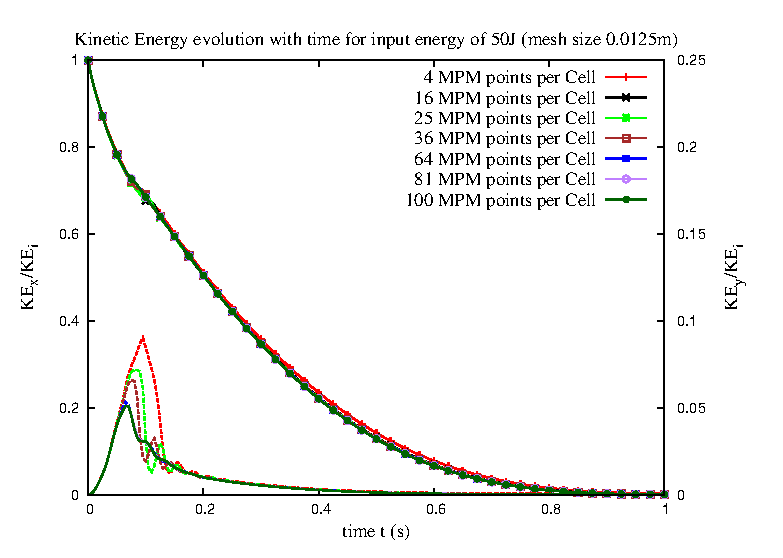
\includegraphics[width=\textwidth]{KE_50}
\caption{$E_0=12.7mgd$.}
\label{fig:KE_50}
\end{subfigure}
\\
\begin{subfigure}[b]{0.95\textwidth}
\centering
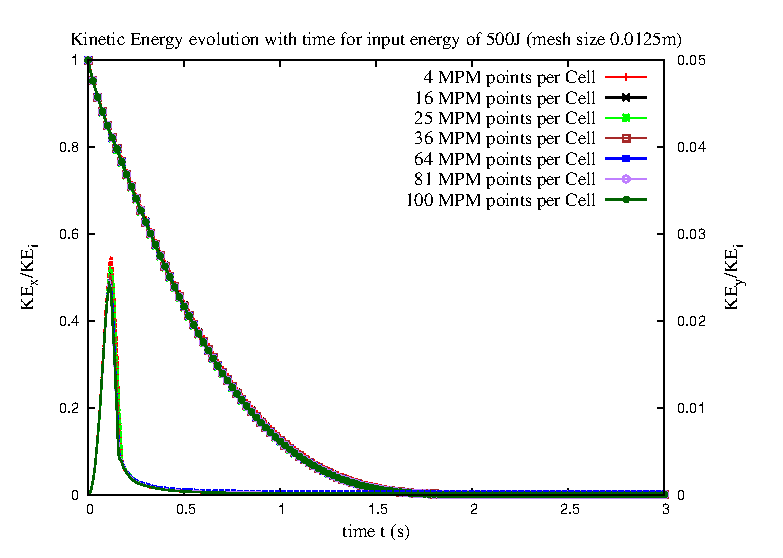
\includegraphics[width=\textwidth]{KE_500}
\caption{$E_0=152mgd$}
\label{fig:KE_500}
\end{subfigure}
\caption{Evolution of kinetic with time for varying material points per cell 
for a slope subjected to an impact velocity.}
\label{fig:KE_MPM}
\end{figure}

The effect of mesh size on the flow kinematics is studied by comparing two mesh 
sizes: 0.01~\si{\m} and 0.0125~\si{\m} (\cref{fig:MPM_Size_Effect}). It can 
be observed that the run-out distance converges with an increase in the number 
of material points per cell in both cases. Less than ~1\% difference in the 
run-out distance is observed between a mesh size of 0.0125~\si{\m} and 
0.01~\si{\m}. The final run-out duration is almost unaffected by the increase 
in the number of material points per cell. 
 

\begin{figure}[tbhp]
\centering
\begin{subfigure}[b]{0.95\textwidth}
\includegraphics[width=\textwidth]{50}
\caption{$E_0=12.7mgd$.}
\label{fig:50}
\end{subfigure}
\\
\begin{subfigure}[b]{0.95\textwidth}
\centering
\includegraphics[width=\textwidth]{500}
\caption{$E_0=152mgd$.}
\label{fig:500}
\end{subfigure}
\caption{Evolution of run-out and duration of flow  for varying material points 
per cell for a slope subjected to an impact velocity.}
\label{fig:MPM_Size_Effect}
\end{figure}

This shows that the run-out distance is affected by the number of material 
points per cell. However, the duration of the run-out is independent of the 
number of material points per cell. The computation time increases with 
increase in the number of material points per cell and decrease in the mesh 
size. However, the run-out distance converges with increase in number of 
material points per cell. Hence, an optimum number of 25 material points per 
cell is adopted in this case. In summary, for conducting a successful MPM 
analysis, a careful selection of the mesh size and the number of particles is 
necessary.

\subsection{GIMPM}

The shape functions used in MPM are continuous, and hence penetration between 
bodies are handled 
automatically without the need for any supplemental contact 
algorithm~\citep{Chen2002}. In MPM, the continuum body deforms and moves in 
an arbitrary computation grid and all the boundary conditions are carried by 
the boundary particles. If a boundary particle is present in a cell, then the 
cell boundary becomes a part of the continuum body, and the cell size 
represents the thickness of the boundary. However, in certain cases both the 
boundary particle and an interior particle can be found in a cell, in which 
case the cell is still treated as a boundary cell, and the interior particle 
temporarily acts as a boundary particle. To avoid numerical errors, it is 
essential to consider smaller cell size along the boundary~\citep{Chen2002}. 

In MPM simulations, numerical noises are observed when the material points 
crosses the cell boundaries as the body deforms, this is termed 
as \textit{cell crossing noise}. If a material point is located very close to 
the cell boundary, it results in discontinuous gradient of the weighing 
function causing a force imbalance on the grid~\citep{bardenhagen2004}. This 
results in large non-physical acceleration values resulting in separation of 
material points from the continuum~\citep{Sulsky1995}. 
~\Cref{fig:cellnoise} illustrates the problem of cell crossing noise. The 
main reason for the occurrence of cell crossing noise is the use of piecewise 
linear shape functions. However, this problem, which is predominant when using 
fine mesh size, can be overcome by changing the order of arithmetic operation 
as proposed by \citet{Sulsky1995}. 

\begin{figure}[htbp]
\centering
\includegraphics[width=0.7\textwidth]{cellnoise}
\caption{Schematic description of occurrence of cell crossing noise in MPM}
\label{fig:cellnoise}
\end{figure}

To overcome the problem of cell crossing 
noise, \citet{bardenhagen2004} proposed an alternate method called the 
Generalized Interpolation Material Point Method that uses smoother shape 
functions and a larger influence region for each grid node. This approach 
minimizes the cell crossing noise. A piecewise-linear grid basis functions are 
written as
%
\begin{align}
\phi{x} = \begin{cases}
1-\left|x\right|/h \qquad &: \qquad \left|x\right| < h \\
0 \qquad &: \qquad otherwise \,,
\end{cases}
\end{align}
where \textit{h} is the grid spacing. The basis function associated with grid 
node \textit{i} at position $x_i$ is then $\phi_i=\phi(x - x_i)$. The basis 
functions in 3-D are separable functions constructed as $\phi_i(x) = \phi_i^x(x)
\phi_i^y(y)\phi_i^z(z)$. GIMP is often implemented using the standard 
piecewise-linear grid basis functions and piecewise-constant particle 
characteristic functions:
\begin{align}
\chi_p = \begin{cases}
1 \qquad &: \qquad \left|x\right| < \frac{1}{2}l_p \\
0 \qquad &: \qquad otherwise \,,
\end{cases}
\end{align}
%
in which case the 1-D MPM and GIMP weighting functions can be grouped together 
in the general form
%
\begin{align}
\phi = \begin{cases}
1 - (4x^2+l_p^2)/(4hl_p)\qquad &: \qquad \left|x\right| < \frac{l_p}{2} \\
1 - \left|x\right|/h \qquad &: \qquad \frac{l_p}{2} \le \left|x\right| < h - 
\frac{l_p}{2} \\
\left(h +\frac{l_p}{2} - \left|x\right| \right)^2/(2hl_p) \qquad &: \qquad h - 
\frac{l_p}{2} \le \left|x\right| < h +
\frac{l_p}{2} \\
0 \qquad &: \qquad otherwise \,,
\end{cases}
\end{align}
%
where $l_p$ is the width of the particle characteristic function 
$\chi_p$.~\cref{fig:gimp} shows a 1-D GIMP weighting function $\bar{\phi}_{ip}$ 
and gradient weighting function $\bar{\nabla\phi}_{ip}$ for a 
piecewise-constant $\chi_p$ with a characteristic length of \textit{l}. The 
GIMP weighting function is smooth, however a discontinuity is observed in the 
gradient weighting function. 


In traditional MPM, boundary conditions only need be applied on those nodes 
which coincide with the extents of the computational domain. As  illustrated 
in~\cref{fig:MPM_Linear} nodes beyond those boundaries are not influenced by 
particles within the domain. This can be considered a result of the zero
width of the Dirac delta characteristic functions. However, special attention 
is required to simulate the boundaries in the Generalized Interpolation 
Material Point Method (GIMP). Namely, because of their increased extents, it is 
possible for particles to influence, and be influenced by, nodes that lie 
outside of the simulation domain (\cref{fig:GIMP_function}). These extra nodes 
are referred to as the ``ghost'' nodes. Boundary condition treatment of these 
nodes for Dirichlet conditions is the same as for the regular boundary
nodes, namely, their computed values are replaced by prescribed 
values~\citep{Steffen2008}.

\begin{figure}[tbhp]
	\centering
	\begin{subfigure}[b]{0.7\textwidth}
	\centering
	\includegraphics[width=0.9\textwidth]{gimp}
	\caption{Example GIMP weighting function $\bar{\phi}_{ip}$ ,
	and gradient weighting function $\bar{\nabla\phi}_{ip}$ centered at 0 using 
	piecewise linear grid basis functions and piecewise constant particle 
	characteristic functions $\chi_p$. Dotted lines denote breaks in the 
	continuity
	of the functions.}
	\label{fig:gimp}
	\end{subfigure}\\
	\begin{subfigure}[b]{0.9\textwidth}
		\centering
		\includegraphics[width=0.9\textwidth]{GIMP_function}
		\caption{GIMP}
		\label{fig:GIMP_function}
	\end{subfigure}\\
	\begin{subfigure}[b]{0.9\textwidth}
		\centering
		\includegraphics[width=0.9\textwidth]{MPM_Linear}
		\caption{Piecewise-Linear}
		\label{fig:MPM_Linear}
	\end{subfigure} 
	\caption{Schematic view of 1-D basis functions used in 
	MPM~\citep{Steffen2008}.}
	\label{fig:MPM_GIMP_func}
\end{figure}

In the present study, the influence of GIMP method on the run-out behaviour of 
a granular column collapse experiment is investigated. A granular column of 
height $H_0$ and length $L_0$ is allowed to collapse and flow on a horizontal 
plane (\cref{fig:exp}). The run-out distance observed is proportional to the 
initial aspect ratio of the column ($H_0/L_0$). Further details about the 
granular collapse experiment and the material properties used in the 
simulations are presented in~\cref{sec:dry_granular_column}. A 
granular column with an initial aspect ratio of 0.4 is considered for the 
comparison. The granular column is represented by 32,000 material points 
arranged uniformly on a regular lattice with a particle spacing of 
0.25~\si{\mm}. A grid size of 1~\si{mm} is adopted with 16 material points per 
cell. In order to understand the influence of the number of material points on 
the accuracy of the solution, simulation using 4 material points per cell with 
GIMP is also performed. The granular collapse experiment is performed for a 
column with an initial aspect ration of 0.4 using both GIMP method and MPM with 
16 material points per cell. 

The evolution of run-out at time $t=\tau_c$ and $t=6\tau_c$, where $\tau_c$ is 
the critical time when the potential energy is fully mobilised, are presented 
in~\cref{fig:MPM_GIMP_TC}. At the initial stage of collapse $t=\tau_c$, both 
MPM and GIMP give almost the same behaviour. The run-out observed in the case 
of 4 material points per cell is similar to the run-out behaviour for 16 
material points per cell. At the end of the flow, GIMP with 4 material points 
show oscillations at the flow front due to fewer material points in a cell. 
However, both MPM and GIMP show a more smoother response at the flow front. The 
evolution of run-out and height with time for both MPM and GIMP are presented 
in~\cref{fig:MPM_GIMP}. For a time up to $t=1.5\tau_c$ all approaches yield the 
exact same behaviour. However, as the flow progresses, the number of material 
points per cell at the flow front decreases and this results in oscillations. 
The oscillations with decrease in the number of material points can be seen in 
the 4 material points per cell. Hence, it is essential to have a larger number 
of material points, especially at the flow front. The difference in the 
normalised run-out between MPM and GIMP method is about 2.5\%. This is due to 
the difference in the interpolation scheme adopted in both approaches. GIMP 
method offers a better approximation of the run-out behaviour as a result of 
the continuous basis function. This also results in a more smooth stress and 
velocity distribution in GIMP than MPM. With increase in the number of material 
points and the use of finer mesh size decrease the difference between both 
approaches. The computational effort using GIMP method is almost twice that of 
MPM, since GIMP method considers the particles at neighbouring cells due to the 
larger spread of the basis functions. In the present study, a very fine mesh 
and 16 material points per cell are used to simulate large deformation 
problems. 

\begin{figure}
	\centering
	\begin{subfigure}[b]{\textwidth}
		\centering
		\includegraphics[width=\textwidth]{4GIMPM_tc}
		\caption{GIMP method (4 material points per cell)}
		\label{fig:4GIMPM_tc}
	\end{subfigure} \\
	\begin{subfigure}[b]{\textwidth}
		\centering
		\includegraphics[width=\textwidth]{16GIMPM_tc}
		\caption{GIMP method (16 material points per cell)}
		\label{fig:16GIMPM_tc}
	\end{subfigure} \\
	\begin{subfigure}[b]{\textwidth}
		\centering
		\includegraphics[width=\textwidth]{16MPM_tc}
		\caption{Conventional MPM (16 material points per cell)}
		\label{fig:16MPM_tc}
	\end{subfigure}
	\caption*{Evolution of granular column collapse at $t = \tau_c$.}
\end{figure}

\begin{figure}
\ContinuedFloat
	\centering
	\begin{subfigure}[b]{\textwidth}
		\centering
		\includegraphics[width=\textwidth]{4GIMPM_6tc}
		\caption{GIMP method (4 material points per cell)}
		\label{fig:4GIMPM_6tc}
	\end{subfigure} \\
	\begin{subfigure}[b]{\textwidth}
		\centering
		\includegraphics[width=\textwidth]{16GIMPM_6tc}
		\caption{GIMP method (16 material points per cell)}
		\label{fig:16GIMPM_6tc}
	\end{subfigure} \\
	\begin{subfigure}[b]{\textwidth}
		\centering
		\includegraphics[width=\textwidth]{16MPM_6tc}
		\caption{Conventional MPM (16 material points per cell)}
		\label{fig:16MPM_6tc}
	\end{subfigure}
	\caption*{$t = 6\tau_c$}
	\caption{Comparison between GIMP method and conventional MPM on the flow 
	morphology of a granular column collapse (a = 0.4).}
	\label{fig:MPM_GIMP_TC}
\end{figure} 

\begin{figure}[tbhp]
	\centering
	\begin{subfigure}[b]{0.95\textwidth}
		\centering
		\includegraphics[width=0.95\textwidth]{Runout_MPM_GIMPM}
		\caption{Evolution of run-out (GIMP method vs MPM)}
		\label{fig:Runout_MPM_GIMPM}
	\end{subfigure} \\
	\begin{subfigure}[b]{0.95\textwidth}
		\centering 
		\includegraphics[width=0.95\textwidth]{Height_MPM_GIMP}
		\caption{Evolution of height (GIMP method vs MPM)}
		\label{fig:Height_MPM_GIMP}
	\end{subfigure} \\
	\caption{Comparison between GIMP method and conventional MPM on the 
	evolution of run-out and height with time for a granular column collapse (a 
	= 0.4).}
	\label{fig:MPM_GIMP}
\end{figure}


\subsection{Application of MPM in geomechanics}

The studies on using the material point method in modelling
geotechnical problems are limited. The potential of Material Point Method in 
modelling granular flows, discharge of silos, was first recognised 
by~\citet{Wieckowski1999}.~\citet{Bardenhagen2001} developed a frictional 
contact algorithm to model granular materials. The Mohr-Coloumb is used to 
describe the kinematics of the grains. In this model, a contact is defined when 
the nodal velocity interpolated from all material points in the cell differs 
from the nodal velocity interpolated from a single material 
point.~\citet{Coetzee2005} applied this contact algorithm to understand the 
pull-out behaviour of anchors.~\citet{Ma2014} developed a new contact algorithm 
with a penalty contact function and a limited maximum shear stress for 
soil-structure interaction, i.e, interaction of pipe-line with debris flow or 
submarine landslide. The penalty contact function behaves similar to numerical 
damping and thus reduces the oscillations during the impact. 

\citet{Beuth2010} applied Gaussian integration in quasi-static MPM to model 
large strain problems. However in this approach, the conservation mass is not 
valid as a larger filled volume of material is considered.~\citet{Andersen2010} 
used GIMP method with an elasto-plastic model to simulate slope failures. The 
solution is found to be dependant on the number of material points used to 
describe the slope geometry.~\citet{Mast2014} studied the behaviour of granular 
column collapse using a non-associative flow rule. They observed a 
significant increase in the run-out distance for large aspect ratio 
columns.~\citet{Mast2014a} investigated the suitability of Material Point 
Method is realistic prediction of large deformation problems such as snow 
avalanches. 

~\citet{Guilkey2007} developed a coupled numerical scheme for fluid-structure 
interaction. The solid field is modelled in a Lagrangian frame, while an 
Eulerian frame, compressible CFD, is used for the fluid. As MPM computation 
grid is reset at every stage, the same Eulerian grid is adopted for both the 
solid and the fluid. Similar approach was adopted by~\cite{Zhang2008} to model 
multiphase flows, where the interactions between the solid and gas are modelled 
using MPM background mesh as an Eulerian 
grid.~\citet{Mackenzie-Helnwein2010} investigated various techniques to model 
multiphase drag forces. Both solid and the fluid are modelled as Lagrangian 
particles using the mixture theory.~\citet{Abe2013} developed a soil–pore fluid 
coupled MPM algorithm based on Biot’s mixture theory for solving 
hydro-mechanical interaction problems. ~\citet{Bandara2013} developed a unique 
approach in modelling solid-fluid interactions. Two sets of Lagrangian 
particles are used to represent soil skeleton and pore water, 
separately.~\citet{Bandara2013} applied the coupled MPM to solve large 
deformation problems such as slope failure due to seepage.

In the present study, the Material Point Method is used to model large 
deformation problems, such as collapse of dry columns and soil slopes subjected 
to impact loading. The suitability of continuum approach (MPM) in modelling 
large deformation problems is also investigated.

\section{Particulate modelling of granular flows}

Granular materials often exhibit different behaviour under different 
circumstances. Fluidized granular material often resembles a liquid, and 
reveals surface waves. In certain situations, granular materials behave more 
like a solid exhibiting plastic deformations. Despite the wide variations in 
the physical and the chemical properties of the grains, the discrete granular 
structure has a rich generic phenomenology, which motivates us to understand 
the fundamental behaviour of these materials. 

A granular material can be 
considered as a continuous material if it is viewed at a macroscopic scale, 
ignoring the fact that it is composed of grains. On a macroscopic scale, the 
behaviour of the granular material could be approximately defined using 
continuum mechanics. However, on a grain level, the granular materials 
exhibit complex solid-like and/or fluid like behaviour depending on the way the 
grains interact with each other. The analytical and finite element models, 
which consider granular materials as a continuum cannot take into account the 
local geometrical processes that govern the mechanical behaviour of a 
non-homogeneous soil. The application of continuum models to describe the 
granular flow poses subtle problems for statistical analysis~\citep{Mehta1994}. 
The grain level description of the granular material enriches the macro-scale 
variables, which poorly account for the local rheology of the materials. 

Numerical models such as the Discrete Element approach proposed 
by~\citet{Cundall1979a} are capable of simulating the granular material as a 
discontinuous system. Although, modern measurement techniques can probe into 
the local granular variables, like grain position, velocities, contact 
forces, etc., they have inherent limitations in acquiring those variables. The 
\textit{discrete-element} approach is a powerful and a reliable research tool 
to study the behaviour granular materials at the grain-scale. This approach 
involves applying Newton's equation of motion simultaneously to all grains 
described as rigid solid bodies by considering the contact forces and the 
external forces acting on the grains. For a given boundary condition, the 
collective mechanical response of grains to the external force leads to the 
relative motion between grains constrained in a dense state and/or by 
in-elastic collisions in the loose state.~\citet{Cundall1979a} applied this 
method to granular geomaterials, and called it the \textit{Distinct Element 
Method}, to differentiate from the existing \textit{Finite Element Method} used 
in geomechanics. The attribute ``distinct'' refers to the degrees of freedom of 
individual grains, but it was later replaced by ``discrete'' to underline 
the discrete nature of the system. 

The interactions between the individual grains are governed by unilateral 
contact laws, and the mechanism of energy dissipation is through friction and 
inelastic collisions. Moreover, granular materials have a wide variation in 
their grain shape and size distribution that require appropriate numerical 
treatments. In DEM, the normal reaction force, 
which prevents the interpenetration of two grains is proportional to the depth 
of penetration. Thus, frictional contact between grains can be expressed 
as a function of the configuration variables, which describe the positions and 
velocities of the grains~\citep{Radjai2011}.

Discrete-Element methods, which describe interactions between grains based on 
the explicit overlap between the grains are termed as \textit{smooth methods}. 
Another approach is the \textit{non-smooth approach}~\citep{Jean1999}, which 
describes the behaviour of discrete elements using the main features of 
uni-laterality and Coulomb friction, and by neglecting the finer details such 
as interpenetration and overlap between grains. The fundamental difference 
between the non-smooth method and the common discrete element method 
lies in the treatment of small length and time scales involved 
in the dynamics of granular media. In DEM, the grains are treated 
as rigid bodies but the contacts between grains are assumed to obey the 
visco-elastic constitutive law. The time-stepping schemes used for the 
numerical integration of the equations of motion in DEM, 
imply that the contact interactions involve smaller time and length scales. In 
the non-smooth Contact Dynamics (CD) method, these small scales are neglected 
and their effects are absorbed into the contact laws. In non-smooth 
formulation, the grain dynamics is described at a larger scale than the elastic 
response time and displacement scales~\citep{Jean1999, Radjai2009}. 

DEM simulations can easily capture the complex flow mechanics of 
large-deformation problems than the continuum approach.~\cite{Tang2009} used 2D 
discrete element modelling to understand the mechanism of the Tsaoling 
landslide triggered by the Chi-Chi earthquake. The authors were able to 
establish the landslide characteristics to have a low-friction coefficient 
(about 0.15) and a medium strength. They were also able to back-calculate a 
maximum velocity of sliding reached 50~\si{\m\per\s}. 
Similarly,~\cite{Tang2013} performed 3D discrete-element simulations to 
understand the 
transportation and deposition of the 2009 Hsiaolin landslide. The authors 
estimated the friction coefficient of landslide-mass to have reached a critical 
value of 0.1, at which the mass begins to slide and reach a maximum velocity of 
40 - 50~\si{\m\per\s}. Two-dimensional DEM simulations have been used to 
analyze the temporal and spatial evolution of slope failure and landslides from 
the intact, pre-failure slope to the restabilized, post-failure slope composed 
of bonded material~\citep{Katz2014}. The pre-failure slope material 
disintegration is found to be the fundamental element in determining the size 
and geometry of the resultant landslides.~\citet{Liu2013} studied the 
kinematics and internal deformation of granular slopes, which experience 
flow-like behaviour. They observed that the Dilatant grain-shearing flow to be 
the dominating mechanism in the movement of granular slopes. DEM is capable of 
probing the material response in a detailed scale, where conventional 
experiments or field tests are not feasible. Hence, in the present study, 2D 
discrete element simulations are performed to understand the behaviour of 
granular flows. 

 
%*******************************************************************************

\section{Discrete Element Method}

Discrete Element Method computes the equilibrium and the trajectories of a 
classical multi-body system. The Discrete Element Method is a simple and 
flexible discrete-element approach, which involves applying Newton's second law 
of motion to each grain to describe the deformation of the granular assembly. 
% 
\begin{equation} 
{m}_{i}\frac{{{d}^{2}}{{x}_{i}}}{d{{t}^{2}}} = {{\mathbf{F}}_{i}}, 
(i=1,...,N ) \,,
\label{eq:fma}
\end{equation}
%
where \textit{N} is the number of grains in the simulation, $m_{\mathit{i}}$ 
is the mass of a grain \textit{i}, $x_{\mathit{i}}$ is its position, and 
$\mathbf{F}_{\mathit{i}}$ is the force exerted on grain. The method consists of 
calculating the forces $\mathbf{F}_{\mathit{i}}$ and then solving 
the ordinary differential in~\cref{eq:fma}. In general the system of coupled 
non-linear differential equations cannot be solved analytically. The 
approximate numerical solution of these equations, which describes the 
trajectories of all the grains of the system is called as Discrete Element 
Method.

DEM simulations are identical to the real experiments, this involve generation 
of samples (initial conditions) with \textit{N} grains and solving the Newton's 
equation of motion for the system until the properties of the system no longer 
change with time (equilibration of the system). After equilibration, the actual 
analysis is performed.

The computation of the forces and torques is the central part of the Discrete 
Element Method simulation. The dynamics of the granular material is governed by 
Newton's equation of motion which depends on the centre-of-mass coordinates and 
the Euler angles of the grains \textit{i} ($i = 1, 2 \cdots , N$):
%
\begin{align} 
\frac{{{\partial}^2}{\overrightarrow{r_i}}}{\partial{t^2}} 
&=\frac{1}{m_i}\overrightarrow{{\mathbf{F}}_{i}}(\overrightarrow{r_j},\overrightarrow{v_j},
 \overrightarrow{\varphi_j},\overrightarrow{\omega_j}) \,, \\ 
\frac{{\partial^2}{\overrightarrow{\varphi_i}}}{\partial{t^2}}&
=\frac{1}{{\hat{J}}_i}\overrightarrow{\mathbf{M}_i}
(\overrightarrow{r_j},\overrightarrow{v_j},\overrightarrow{\varphi_j},
   \overrightarrow{\omega_j}), (j=1,...,N) \,.
\end{align}
%
The force $\overrightarrow{\mathbf{F}_{i}}$ and the torque 
$\overrightarrow{\mathbf{M}_{i}}$, which act on grain \textit{i} of mass 
$\mathit{m}_{\mathit{i}}$ and the tensorial moment of inertia 
${\hat{J}_i}$ are (sometimes complicated) functions of the grain 
positions $\overrightarrow{\mathit{r}_{\mathit{j}}}$, their angular 
orientations $\overrightarrow{\varphi}_{\mathit{j}}$, and their corresponding 
velocities $\overrightarrow{\mathit{v}_{\mathit{j}}}$ and 
$\overrightarrow{\omega}_{\mathit{j}}$. In a two-dimensional system, the 
angular orientation of a grain is described by a single (scalar) quantity 
$\varphi_{i}$ and the moment of inertia reduces to a scalar value 
$\mathit{J}_{i}$. 
%The Newton's equation of motion can be written as
%%
%\begin{align} 
%	\frac{{{\partial}^2}{\overrightarrow{r_i}}}{\partial{t^2}} 
%	
%&=\frac{1}{m_i}\overrightarrow{{\mathbf{F}}_{i}}(\overrightarrow{r_j},\overrightarrow{v_j},
%	\overrightarrow{\varphi_j},\overrightarrow{\omega_j})
%	\nonumber \\ 
%	
%\frac{{\partial^2}{\overrightarrow{\varphi_i}}}{\partial{t^2}}&=\frac{1}{{\hat{J}}_i}\overrightarrow{\mathbf{M}_i}(\overrightarrow{r_j},\overrightarrow{v_j},\overrightarrow{\varphi_j},
%	\overrightarrow{\omega_j}), (j=1,...,N) \,. \nonumber
%\end{align}

For granular grains in the absence of long range fields, the force  
$\overrightarrow{\mathbf{F}_{i}}$ and the torque  
$\overrightarrow{\mathbf{M}_{i}}$ acting upon the grain \textit{i} are given as 
sum of the pairwise interaction of grain \textit{i} with 
all other grains in the system:
%
\begin{align}
   \overrightarrow{{\mathbf{F}}_i}=\sum\limits_{j=1,j\ne 
   i}^{N}{\overrightarrow{\mathbf{F}_{ij}}}, \qquad 
   &\overrightarrow{\mathbf{M}_{i}}=\sum\limits_{j=1,j\ne 
   i}^{N}{\overrightarrow{\mathbf{M}_{ij}}} \,.
\end{align}
%
The limitation to pairwise interaction is an abstraction, which is justified 
if the grains deformation at the contact is trivial. To describe the 
deformation of granular assemblies one has to take into account the effect of 
multi-grain interactions. This method is general and can be applied to a wide 
range of systems. The Discrete Element Method can be used to study the 
behaviour of grains in rapid flows to static assemblies. The method treats 
both the conditions in exactly the same way, it is not necessary to divide the 
system and then treat each condition differently. The simplest model for 
granular grain is a sphere. In a two-dimensions case, the sphere is reduced to 
a circular disk. Simulations using spherical grains are numerically very 
effective since grain collisions can be easily identified and described in 
a simple way~\citep{Poschel2005}.

% 
%%******************************************************************************

\subsection{The Forces}

The force $\mathbf{F}_{\mathit{i}}$ in~\cref{eq:fma} represents both the grain 
to grain interaction force, and other external forces acting on the system. 
Therefore, the force $\mathbf{F}_{\mathit{i}}$ is expressed as
%
\begin{equation} \label{eq:f}
 \mathbf{{F}}_{i}=\sum\limits_{j\ne 1}{\mathbf{{F}}_{ij}+\mathbf{{F}}_{ext, 
 i}}\,,
\end{equation}
%
where $\mathbf{F}_{\mathit{i}}$ is the force exerted by grain \textit{j} on 
\textit{i}. The external force $\mathbf{F}_{\mathit{ext,i}}$ is most often the 
force of gravity, $\mathbf{F}_{\mathit{ext,i}} = m_{\mathit{i}} \mbox{ 
}\mathbf{g}_{\mathit{i}}$. The methodology to incorporate any other external 
forces in the simulation is the same. However, the computation of the 
interaction forces depends on the numerical method adopted in the study. 
The methodology used in the present study is described below. 

Let us consider two grains \textit{i} and \textit{j}, in contact 
(\cref{fig:DEM}). The contact force can be decomposed into two components, 
as the normal ($\mathit{F}_{n}$) and the tangential ($\mathit{F}_{t}$) 
components
%
\begin{equation}
 \mathbf{F}_{ij}=F_{n}\mathbf{n}+F_{t}\mathbf{t} \,.
\label{eq:fnt}
\end{equation}

\begin{figure}[htbp]
	\centering
	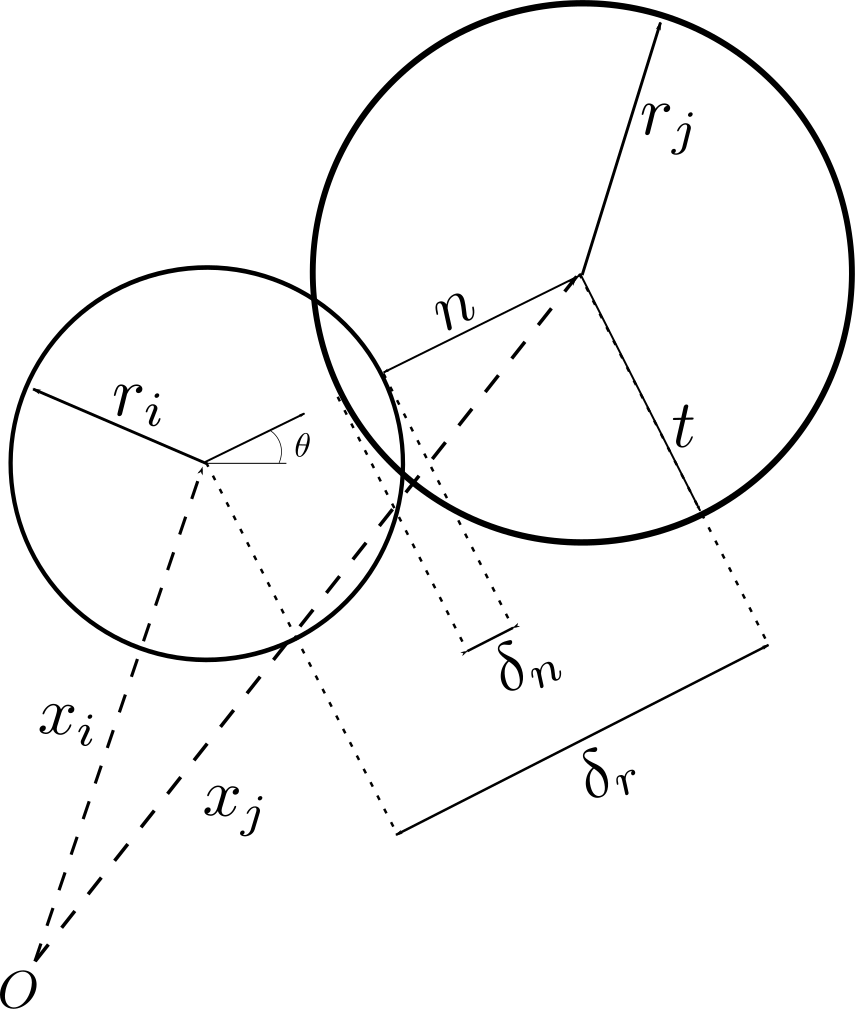
\includegraphics{DEM}
	\caption[Calculation of normal force in DEM]{Grains \textit{i} and 
	\textit{j} in 
	contact, and the 
	separation $\delta_{n}$ is used to calculate the normal force} 
	\label{fig:DEM}
\end{figure}

where \textbf{n} and \textbf{t} are unit vectors, pointing in the normal and 
the tangential directions. The procedure adopted to calculate the normal and 
tangential forces are discussed.

%****************************************** %
\subsubsection*{Normal force}
When grains collide, part of the kinetic energy is dissipated as 
heat and the other part causes deformation of the grain. These deformations 
generate interaction forces. The grains are considered to be rigid while their 
contact is assumed to be soft. Thus, the grains do not change their shape, 
instead they overlap. The shapes of the grains are conserved on an average, 
after many collisions. The overlap at the contact is limited to very small 
deformations, which are achieved by defining a repulsive normal force that 
opposes the overlap. The mutual compression ($\delta_{n}$) of the grains 
\textit{i} and \textit{j} is defined as
%
\begin{equation}
 \delta_{n}=\left|x_{\mathbf{i}}-x_{\mathit{j}}\right|-r_{i}-r_{j} \,,
\label{eq:delta}
\end{equation}
%
where $x_{\mathit{i}}$ and $x_{\mathit{j}}$ are the centres of the grains and  
$r_{\mathit{i}}$ and $r_{\mathit{j}}$ are their radii (\cref{fig:DEM}). When 
$\delta_{n}>0$, the two grains are not in contact, and 
there is no interaction. When $\delta_{n}<0$, the two grains overlap, and 
there is a repulsive normal force that pushes the two grains apart. The 
simplest model is to consider the contact as a linear spring with damping. The 
repulsive force depends linearly on $\delta_{n}$, and is controlled by the 
stiffness of the grain. The energy dissipation due to the interaction between 
grains is an intrinsic characteristic of the granular material and is 
incorporated by adding a damping force that opposes the relative velocity for 
the duration of the contact. The interaction force at the contact is idealized 
as a simple spring-dashpot system, with elastic and dissipative 
constants~\citep{Luding1994}. 
%
\begin{align}
 {{F}_{n}}=
\begin{cases}
0, & {{\delta}_{n}}>0 \\
-{{k}_{n}}{{\delta}_{n}}-{{\gamma}_{n}}\frac{d{{\delta}_{n}}}{dt}, & 
{{\delta}_{n}}<0 \\
\end{cases}
\end{align} 
%
The constant ${k}_{n}$ characterises the stiffness of the grain, and must be 
chosen sufficiently large so that the overlap between the grains remain small. 
Nevertheless, the solution has an undesirable property of generating an 
attractive force~\citep{Poschel2005}. It arises just before the two grains 
separate. In this case, we have ${d{\delta_{n}}}$$/{dt} > 0$ while $\delta_{n}$ 
approaches zero. To avoid the attractive force, the force is computed in two 
stages: a candidate force $\hat{F}_{n}$ is calculated, and verified whether it 
is non-negative
%
\begin{align}
 {\hat{F}_{n}}=-{{k}_{n}}{{\delta}_{n}}-{{\gamma}_{n}}\frac{d{{\delta}_{n}}}{dt},
  \quad F_{n}=
\begin{cases}
0, & {\hat{F}} \le 0 \\
{\hat{F}}_{n}, & {\hat{F}} > 0 \\
\end{cases} \label{eq:nf}
\end{align} 
%
For pairwise collisions, the normal force $(F_{n})$ represented as 
${{k}_{n}}{{\delta}_{n}}+{{\gamma}_{n}}$ causes a decrease in the relative 
normal velocity of the grains by a factor $\varepsilon$. This factor is the 
\textit{coefficient of restitution}, and is defined as $\varepsilon\approx 
g'/g$, 
where \textit{g} is the absolute normal relative velocity before 
the collision and \textit{g'} corresponds to the post-collision value. The 
relative velocity, ${d{\delta_{n}}}$$/{dt} > 0$, can be obtained by 
differentiating~\cref{eq:delta}. Thus we obtain
%
\begin{equation}
\label{eq:vn}
\frac{d{\delta_{n}}}{dt}=(\mathbf{v}_{\mathit{i}}-\mathbf{v}_{\mathit{i}}).{\mathbf{n}}\,,
\end{equation}
%
where $\mathbf{v}_{\mathit{i}}=dx_{\mathit{i}}/dt$ is the velocity of grain 
\textit{i} and $\mathbf{v}_{\mathit{j}}=dx_{\mathit{i}}/dt$ is the velocity of 
grain \textit{j}. The numerical integration of~\cref{eq:vn} yields the 
separation $\delta_{n}$ and permits us to generalise the model and treat the 
tangential forces as well, as explained in the next section. By integrating 
Newton's equation of motion it is found that the linear force corresponds to 
the co-efficient of restitution, which is defined as
%
\begin{equation}
\varepsilon=exp(-\frac{\pi\gamma_{n}}{2m^{eff}}/\sqrt{\frac{Y}{m^{eff}}
-{\frac{\gamma^{n}}{2m^{eff}}}^{2}})\,.
\end{equation}
% 
%%*************************************************************************************************************************************************
% %

\subsubsection*{Tangential force}
Grains are not perfect spheres, but have a complicated surface 
texture, therefore at oblique collisions, besides the normal force there is a 
tangential force too. Even perfectly smooth spheres exert a tangential force 
due to their bulk viscosity~\citep{Poschel2005}. To build a heap of 
spheres on a flat surface, the grains as well as the surface have to be 
sufficiently rough, indicating the dependence of the tangential force on the 
surface properties of the granular materials. For realistic simulation of 
granular materials, it is important to consider the tangential force in 
DEM. The tangential force is considered in a similar 
fashion as the normal force, arising from a spring stretched by the relative 
motion of the grain. Tangential forces are modelled by considering the relevant 
relative tangential velocity of the grain surfaces at the point of contact. The 
point of contact is an approximation, as the description of the normal force 
assumes a compression $\delta_{n}$, which implies a contact surface in 3-D or a 
contact line in 2-D. Assuming a tangential spring of length $\delta_{t}$ exerts 
an opposing force to the relative tangential displacements (ignoring the effect 
of relative rolling between the grains), the tangential force can be postulated 
similar to the normal force (\cref{eq:vn}) as
%
\begin{equation}
\label{eq:vt}
\frac{d{\delta_{t}}}{dt}=(\mathbf{v}_{\mathit{i}}-\mathbf{v}_{\mathit{i}}).{\mathbf{t}}
 \,.
\end{equation}
%
This equation must also be numerically integrated, just like~\cref{eq:fma}. The 
grains are in contact when $\delta_{t}<0$, and when $\delta_{t}=0$, the grains 
no longer exert a force on each other. With these assumptions, $\delta_{t}$ can 
be calculated similar to the normal force. The tangential force is assumed to 
be governed by Coulomb's friction law.
%
\begin{equation}
\left|F_{\mathit{t}}\right|\le\mu F_{\mathit{n}} \,, \label{eq:fric}
\end{equation}
%
where $F_{\mathit{t}}$ is the tangential force and $\mu$ is the friction 
coefficient. It is therefore necessary to constrain the tangential force to 
remain less than or equal to $\mu F_{N}$. To impose the condition 
in~\cref{eq:fric}, two-stages similar to the normal force computation is 
adopted. The first step is to evaluate the candidate force, and is then 
accepted if it obeys the condition in~\cref{eq:fric}.
%
\begin{align}
 {\hat{F}_{t}}=-{{k}_{t}}{{\delta}_{t}}-{{\gamma}_{t}}\frac{d{{\delta}_{t}}}{dt},
  \quad F_{t}=
\begin{cases}
sgn(F_{t}), & {\left|\hat{F}\right|} \ge \mu F_{n} \\
{\hat{F}}_{t}, & {\left|\hat{F}\right|} < \mu F_{n} \\
\end{cases}
\label{eq:tf}
\end{align} 
%
where $k_{t}$ is the stiffness of the tangential spring and $\gamma_{t}$ is the 
damping constant. If $|F_{t}|=\mu F_{n}$, the contact is sliding, otherwise, it 
is non-sliding. It can noted that the normal force (\cref{eq:nf}) and the 
tangential force (\cref{eq:tf}) are handled in the same way in DEM. When the 
grains slide against each other, they do not retain any memory 
of their initial position, and hence do not return to its original position. In 
order to model this behaviour, a limiting value of $\delta_{t}$ is imposed. 
When the contact slides $\delta_{t}=\pm\mu F_{n}/k_{t}$ is imposed.

In addition to sliding, the grains can roll relative to one another about their 
centre of mass due to the tangential force acting at their contact surface. In 
this case, $d\delta_{t}/dt=0$. It is important to assume that the grains touch 
at a single point instead of overlapping, i.e. $\delta_{n}=0$. This point is 
located at 
${x}_{\mathit{i}}-r_{\mathit{i}}\mathbf{n}={x}_{\mathit{j}}+r_{\mathit{j}}\mathbf{n}$.
 If we consider that this point belongs to grain $\mathit{i}$, its velocity is 
${v}_{\mathit{i}}+r_{\mathit{i}}(\mbox{\boldmath${\omega}$}\times\mathbf{n})$. 
If it belongs to grain \textit{j}, its velocity is 
${v}_{\mathit{j}}+r_{\mathit{j}}(\mbox{\boldmath${\omega}$}\times\mathbf{n})$. 
The relative velocity is the difference between these two velocities. 
%
\begin{equation}
\frac{d\delta_{t}}{dt}=(\mathbf{v}_{\mathit{i}}-{\mathbf{v}}_{\mathit{j}})\cdot 
\mathbf{t} 
-(r_{\mathit{i}} \mbox{\boldmath${\omega}$}_{\mathit{i}}
+r_{\mathit{j}}\mbox{\boldmath${\omega}$}_{\mathit{j}})\times\mathbf{n} \,.
\label{eq:rf}
\end{equation}
%
It should be noted that the~\cref{eq:rf} is only an approximation, as the 
grains in DEM do not touch at points, but overlap. It is therefore an 
approximation that produces an error of order 
$\mathbf{\mathit{O}}(\delta_{n}/r)$~\citep{Radjai2011}. It is 
assumed that the contact forces are exerted at the point of contact. It implies 
that the tangential force is accompanied by torque acting on two grains. If the 
overlap is zero, these torques are
%
\begin{align}
\tau_{\mathit{ij}} & = -(a_{\mathit{i}}\mathbf{n})\times(F_{t}\mathbf{t}) \,,\\
\tau_{\mathit{ji}} & = -(a_{\mathit{j}}\mathbf{n})\times(F_{t}\mathbf{t}) \,.
\label{eq:av}
\end{align}
%
The torques modify the angular velocities of the grains. It is therefore 
necessary to incorporate the equation for the angular coordinates of the grains 
in~\cref{eq:fma}
%
\begin{equation}
\mathit{I}_{j}\frac{d\omega_{i}}{dt}=\sum\limits_{j\ne i}{\tau_{ij}} \,,
\end{equation}
%
where $\mathit{I}_{j}$ is the moment of inertia of grain j. The~\cref{eq:av} is 
only valid when $\delta_{n}=0$. The torque is a vector product of the force and 
its lever arm. It is assumed that the lever arms have lengths equal to 
$r_{\mathit{i}}$ and $r_{\mathit{j}}$, which is true only when the grains do 
not overlap, hence in this case they produce an error of order 
$\mathbf{\mathit{O}}(\delta_{n}/r)$. It is nevertheless desirable to damp this 
type of motion~\citep{Radjai2011}. 


The interaction between two solid bodies is much more complex than that is 
described by the simple linear model. Nevertheless, the linear force law has 
several advantages. It is simple to implement, and its harmonic behaviour is 
well understood, which makes it easier to interpret the results. The 
most common non-linear interaction law is the Hertz law~\citep{Hertz1882}. In 
certain situations, such as a quasi-static packing, a non-linear law can have 
significant influence on the acoustic properties, and on the global 
stiffness~\citep{Agnolin2007}. However, in case of rapid granular flows, 
the interaction force between the grains has almost no effect on the 
phenomenon, and a linear law can be used to describe this kind of 
behaviour~\citep{Radjai2011}. 

%****************************************************************************

\subsection{Numerical algorithm and integration scheme}
The efficiency of a DEM algorithm is mainly determined by 
its efficiency to compute the interaction forces between grains. If we 
consider a model system with pairwise interactions, we have to consider the 
contribution of the force on grain \textit{i} due to all its neighbours. If we 
consider only the interaction between a grain and the nearest image of another 
grain, then for a system of \textit{N} grains, we must evaluate $N \times 
(N-1)/2$ pair distances. Consider a system of 1000 grains, at every time step 
all possible pairs of grains have to be considered to compute the interaction 
forces, hence, $\mathit{N}(\mathit{N}-1)/2 \approx 500,000$ force computations 
are required. For short-range grain interactions, the majority of these force 
evaluations is unnecessary as the corresponding grains are located far apart 
and do not necessarily touch each other. For a dense system of equally sized 
grains, the grains can have contacts with not more than 6 grains, this reduces 
the number of force computation required to $3\mathit{N} \approx 3000$. In the 
preliminary force computation scheme, at least 166 times more pair interactions 
are considered than necessary. Therefore, the numerical methods employed in the 
DEM should try to minimize the computation of 
interaction forces~\citep{Poschel2005}. There are three different methods for 
the efficient computation of the forces, the \textit{Verlet} algorithm, the 
\textit{link-cell} algorithm, and a \textit{lattice} algorithm. The 
\textit{Verlet} algorithm described in~\citet{Grubmuller1991} 
is implemented in the present study.

\subsubsection{Verlet list algorithm}
The Verlet list algorithm assumes a cut-off value, so that only neighbouring 
grains that contribute to the energy of a grain \textit{i} are considered. It 
is advantageous to exclude the grains that do not interact in the memory 
expensive energy computation.~\citet{Verlet1967} developed a book-keeping 
technique, commonly referred to as the Verlet list or neighbour list, which is 
illustrated in~\ref{fig:Verletb}. In this method a second cut-off radius 
$r_{\mathit{v}}>r_{c}$ is introduced, and before the interactions are 
calculated, a list is made (the Verlet list) of all grains within a radius 
$r_{\mathit{v}}$ of the grain \textit{i}. In the subsequent calculations of the 
interactions, only those grains in this list will be considered. The idea of 
the Verlet algorithm is based on a simple property of grain dynamics: 
neighbourhood relation between grains can only change slowly, i.e. two grains 
which are close to each other at a given time step will remain as neighbours, 
at least in the following few time steps. During initialization the 
neighbourhood relations between the grains, i.e. the distance of all close 
pairs of grains are computed. Two grains are considered as neighbours if 
the distance of their surface is smaller than a predefined distance 
\textit{Verlet distance}
%
\begin{equation}
(\left|\overrightarrow{r_{\mathit{i}}}-\overrightarrow{r_{\mathit{j}}}\right|
-\mathit{R}_{\mathit{i}}-\mathit{R}_{\mathit{j}})<\mbox{\textit{Verlet
 distance}} \,.
\end{equation}

\begin{figure}[tbhp]	
\centering
\includegraphics[width=0.5\textwidth]{Verletb}
\caption[Verlet list algorithm for neighbourhood search]{The Verlet list: a 
grain \textit{i} interacts with 
those grains with 
the cut-off radius $r_{c}$, the Verlet list contains all the grains within 
a sphere with radius 
$r_{\mathit{v}>r_{c}}$}
\label{fig:Verletb}
\end{figure}

For each grain there is a \textit{Verlet list} in which the close 
neighbours are saved. To initialise the Verlet lists efficiently, a grid that 
covers the simulation area is defined. Its mesh size is larger than the largest 
grain. For construction of the lists only pairs whose grains reside in the same 
or adjacent grids are considered. This procedure guarantees the detection of 
all close pairs of grains~\citep{Poschel2005}. Redundancy in Verlet lists, i.e. 
if grain \textit{i} is a neighbour of \textit{j}, then grain \textit{j} is 
a neighbour of \textit{i}, are avoided by imposing a restriction on the list of 
grain \textit{i} contains, such that it contains only neighbours with index 
$\mathit{j}<\mathit{i}$. For the computation of interaction forces, the Verlet 
list of grain \textit{i} is scanned and only pairs which are recorded in one of 
the Verlet lists are considered. Hence, the Verlet list of each grain 
\textit{i} is scanned and the interaction force of \textit{i} with each entry 
\textit{j} in its list is computed. 

Initially to build the Verlet list, the grains are sorted into a grid of mesh 
size $\mathit{dx}\times\mathit{dy}$. For each grid there is a list of grains 
residing in the cell. During the simulation, the neighbourhood relation among 
the grains change, therefore, the Verlet lists have to be updated. The decision 
to update a Verlet list depends on how far the grains have travelled since the 
time when the present list was built. The Verlet list of a grain \textit{i} 
must contain at any time all neighbours \textit{j} with 
$\mathit{j}<\mathit{i}$. This assures that two grains \textit{i} and 
\textit{j} never touch and are not considered as neighbours, i.e. \textit{j} is 
not in the list of \textit{i} and \textit{i} is not in the list of \textit{j}. 
Hence,
%
\begin{equation}
\left|\overrightarrow{r_{\mathit{i}}}-\overrightarrow{r_{\mathit{j}}}\right|
-\mathit{R}_{\mathit{i}}-\mathit{R}_{\mathit{j}}>0 \,.
\end{equation}

The above condition is required for all pairs $(\mathit{i},\mathit{j})$ of 
grains which are \textit{not} known as neighbours. This condition is a 
criterion to update the Verlet lists~\citep{Poschel2005}. Assume at the instant 
when the Verlet lists are constructed, the surfaces of the grains have the 
distance $\left| \overrightarrow{r_{\mathit{i}}} - 
\overrightarrow{r_{\mathit{i}}}\right| - 
\mathit{R}_{\mathit{i}}-\mathit{R}_{\mathit{j}} > 
\mbox{Verlet distance}$, i.e. they are not classified as neighbours. If the 
Verlet lists are updated before one of these grains has travelled the distance 
$\mathit{verlet distance}/2$ since the lists were constructed, they can never 
collide without being recognized as neighbours first. This is explained 
in~\cref{fig:Verlet}. The impact of optimisation of the Verlet list 
algorithm has negligible effect on the computation time, as the algorithm is 
quite efficient already and only consumes a few percent of the total 
computation time in construction of the Verlet lists. The implementation of the 
Verlet list algorithm in force computation drastically reduces the computation 
time in comparison to the linear algorithm. The performance of the Verlet list 
algorithm is controlled by two crucial parameters: the number of cells 
$\mathit{N}_{\mathit{c}}$, for the construction of the Verlet lists and the 
Verlet distance $r_{\mathit{v}}$~\citep{Poschel2005}.

\begin{figure}[htbp]
\centering
\includegraphics[width=0.975\textwidth]{Verlet}
\caption[Checking the validity of Verlet list in DEM simulations]{Checking the 
validity of Verlet 
lists. \textit{Left}: the grains \textit{i} and \textit{j} are not recognized 
as neighbours since the distance of their surface is larger than the Verlet 
distance. The radius of the dashed circle is 
$\mathit{R}_{\mathit{i}}+\mathit{R}_{\mathit{max}}+\mbox{\textit{Verlet 
distance}}$. \textit{Right:} in the most unfortunate case the grains approach 
each other directly, travelling at the same velocity. As soon as one of the 
grains has travelled the distance $\mbox{\textit{Verlet distance}}/2$ 
(\textit{arrows}), the Verlet lists have to be rebuilt. The grains \textit{i} 
and \textit{j} are now recognized as neighbours. Redrawn 
after~\citet{Poschel2005}.}
\label{fig:Verlet}
\end{figure}

\subsubsection{Leap frog or Verlet integration algorithm}

Discrete Element Method involves numerically solving Newton's equation of 
motion~\cref{eq:fma}, which is an ordinary differential equation. Choosing an 
integration algorithm is important, as the forces are not always differentiable 
in time, and the temporary derivative of the force is discontinuous when the 
contact splits. It is also very essential to numerically integrate~\cref{eq:rf} 
with the same precision as~\cref{eq:fma}. At first, computational speed seems 
important. It is usually not very relevant because the fraction of time spent 
on integrating the equation of motions (as opposed to computing the 
interactions) is small. Accuracy for large time steps is more important, 
because the larger the time step that we can use, the fewer evaluation of the 
forces are needed per unit of simulation time. Hence, this would suggest that 
it is advantageous to use a sophisticated algorithm that allows use of larger 
time step. 

Algorithms that allow the use of large time steps, achieve this by storing 
information on increasingly higher-order derivatives of the 
grain coordinates. Consequently, they tend to require more memory storage. 
However, the most important aspect to consider is the energy conservation. It 
is important to distinguish between two kinds of energy conservation: the short 
time and long time. The sophisticated higher-order algorithms tend to have very 
good energy conservation at short times. However, they often have undesirable 
feature that results in drifting of the overall energy for longer times. In 
contrast, the Verlet style algorithms tend to have only moderate short term 
energy conservation, but little long-term drift~\citep{Frenkel1996}. In this 
case, such algorithms are not useful. They are more complicated to program, and 
do not yield a more precise solution~\citep{Radjai2011}. It might seem 
important to have an algorithm that accurately predicts the trajectories of 
all grains for both short and long durations, however no such algorithm exists.


In certain cases, two trajectories that are initially very close may diverge 
exponentially as time progresses. Any integration error, however small it may 
be, would always diverge the predicted trajectory exponentially from the true 
trajectory. This phenomenon is called the Lyanpunov instability, and it is 
devastating to the whole idea of Discrete Element Method simulation, but we 
have good reasons to assume that even this problem need not be 
serious~\citep{Frenkel1996}. First of all, one should realize that 
the aim of DEM is not to predict precisely what will happen to a system, but 
to predict the average behaviour of the system that is prepared in an initial 
state about which we know something (initial position, velocity and energy), 
but not everything. Hence, DEM differs from other methods, which are used to 
predict the trajectories. However, considerable numerical evidence suggest that 
the shadow orbits exists, which is a true trajectory of a multi-body system 
that closely follows the numerical trajectory for a time that is longer in 
comparison with the time that is required for the Lyapunov instability to 
develop~\citep{Frenkel1996}.

Newton's equations of motion are time reversible, and so should be the 
integration algorithm. The ``leapfrog'' algorithm or the Verlet integration 
algorithm is a numerical scheme used to integrate the Newton's equation of 
motion to calculate the trajectories of grains and is implemented in 
DEM by~\citet{Verlet1967}. Verlet algorithm is 
fast and requires less storage memory, it is not particularly accurate for long 
time steps, and hence, we should expect to compute the forces on all grains 
rather frequently. Its short-term energy conservation is fair (in versions that 
use more accurate expression for velocity), but most importantly it exhibits 
little long-term energy drifts. This is related to the fact that the Verlet 
algorithm is time reversible and area preserving, however, it does not conserve 
the total energy of the system exactly~\citep{Frenkel1996}. Verlet algorithm is 
simply based on a truncated Taylor expansion of grain co-ordinates. 
%
\begin{equation}
t(t+\Delta t)=r{t} +\mathbf{v}(t) \Delta t + \frac{f(t)}{2\mathit{m}} \Delta 
t^{2}+ \dots
\end{equation}
%
If we truncate this expansion beyond the term $\Delta t^{2}$, we obtain the 
Euler's algorithm, which looks similar to the Verlet Algorithm, but it does not 
preserve energy and have significant energy drifts. The simplest among the 
Verlet schemes is the \textit{Leap frog algorithm}, which evaluates the 
velocities at half-integer time steps and uses these velocities to compute the 
new positions. The position of each grain is calculated at time $t=0, \Delta t, 
2\Delta t, $\dots$ ,$ where $\Delta t$ is the time step. On the other hand, 
their velocities are calculated at intermediate times, that is, at $t=\Delta 
t/2, 3 \Delta t/2, \dots,$. Let the position of a grain at time $t=k\Delta t$ 
be written as $x_{\mathit{k}}$, and its velocity at time $t=\Delta t (k + 
1/2)$ be written $\mathbf{v}_{\mathit{k + 1/2}}$, and its acceleration at $t=k 
\Delta t$ be $\mathbf{a}_{\mathit{k}}$. Then the following equation is used to 
advance systematically
%
\begin{align}\label{eq:verlet}
\mathbf{v}_{\mathit{k}+1/2} & 
=\mathbf{v}_{\mathit{k}-1/2}+\mathbf{a}_{\mathit{k}}
 \Delta t, \\
x_{\mathit{k}+1} & =x_{\mathit{k}}+\mathbf{v}_{\mathit{k}+1/2} \Delta t
\end{align}
%
This algorithm determines the new grain position with an error of order 
$\mathit{O}( \Delta t^{4})$. But~\cref{eq:verlet} hides a difficulty in the 
application of this algorithm to granular materials~\citep{Radjai2011}. The 
problem is that the acceleration must be calculated at time $t=k\Delta t$. But 
the velocities are known at $t=(k - 1/2) \Delta t$, and not at $t=k \Delta 
t$. One way to get around this problem is to write
%
\begin{equation} 
\mathbf{v}_{\mathit{k}}={\mathbf{v}_{\mathit{k}-1/2}+{\mathbf{a}_{\mathit{k}-1}\Delta
 t/2}} \,.
\label{eq:ver}
\end{equation}
%
The equation uses the acceleration of the preceding time step to estimate the 
velocity. This approximation does not diminish the order of the 
algorithm.~\cref{eq:ver} estimates $\mathbf{v}_{k}$ with an error of order 
$\mathbf{O}(\Delta t^{2})$, which produces an error of the same order in the 
calculation of the force in~\cref{eq:verlet}. But this causes only an error of 
order $\mathbf{O}(\Delta t^{3})$ in the velocity and an error of order 
$\mathbf{O}(\Delta t^{4})$ in the position. However, this problem does not 
exist in energy conservation systems, because the computed forces do not depend 
on the velocities of the grains. The heaviest computational task is the 
evaluation of forces and not the integration of equations. The Verlet 
integration scheme is summarized in~\cref{eq:vers} and~\cref{fig:verlet}. To 
calculate the forces and acceleration, it requires the positions and velocities 
at time \textit{t}:
%
\begin{align}
\mathbf{v}(t+\Delta t/2) & =\mathbf{v}(t-\Delta t/2) + \mathbf{a}(t) \Delta t 
\nonumber \,, \\
x(t+\Delta t) & = x(t)+\mathbf{v}(t+\Delta /2) \Delta t  \,, \nonumber \\
 \mathbf{v}(t) & = \mathbf{v}(t-\Delta t /2)+\mathbf{a}(t- \Delta t) \Delta t 
 /2 \,.
\label{eq:vers}
\end{align}

\begin{figure}[tbhp]
\centering
\includegraphics{Leap}
\caption{Verlet integration scheme}
\label{fig:verlet}
\end{figure}

The analysis of the Discrete Element Method formulation reveals that the linear 
force law gives the model a harmonic character, showing that it is very closely 
related to simple models widely used in physics and mechanics. The shortest 
time scales often arise from the oscillations of one or two grains. The 
integration algorithm must resolve these movements with sufficient precision. 
Thus, the time steps used must be smaller than these time scales, the most 
rapid frequency is usually ${\omega}_{\mathit{N}}$, the characteristic 
oscillation frequency of very short waves. This frequency is proportional to 
$\omega _{o}$, which is easier to estimate. Therefore, it is essential 
to choose a time step $\Delta t \approx \epsilon / \omega_{0}$, where 
$\epsilon$ is a constant that depends on the integration algorithm. Values such 
as $\epsilon \approx 0.01$ are often a reasonable choice~\citep{Radjai2011}. In 
the case of rapid granular flows, the time step must be small enough so that 
the fastest grains move only by a small fraction of their size during one 
time step. The grains must be stiff enough so that violent collisions do not 
lead to large overlaps between grains. 

%%********************************************************************************


\subsection{Boundary conditions}

In many cases, the dynamic and static properties of a granular system are 
substantially affected by the interaction of the granular material with the 
system boundaries, i.e. by the properties of the container or the surface on 
which the material is present. The effect of boundary conditions on 
the response of the granular assembly can be noticed in the convective motion 
of granular material in vibrating containers, the formation of density waves in 
pipes, the motion of granular material on conveyors, and the clogging of 
hoppers. In these and many other cases, careful definition of the interaction 
between the granular material and the contact surface is essential. Of 
particular importance is the realistic modelling of the wall surface roughness. 
Unfortunately the mechanical interaction of a granular materials with a rough 
wall is poorly understood~\citep{Poschel2005}. A simple way to define the wall 
property is to build up the wall from grains, which obey the same rules of 
interaction as the grains of granular material. By varying the size and 
position of the wall grains, system boundaries of adjustable roughness can be 
described. However, the surface roughness that characterizes the frictional 
properties of the wall has to be arrived iteratively, and may not represent the 
real conditions. In the present case, a solid wall with corresponding 
stiffness, damping and frictional characteristics is introduced to model the 
interaction between grains and the wall. The interaction force is computed in a 
similar fashion to that of a pair of grains in contact and is divided into the 
normal and tangential components. The compression of the grain upon collision 
with the wall is calculated along the normal direction to the wall and 
the grain contact.

\subsubsection{Periodic boundary} \label{sec:periodic}
The effect of a wall on the response of grains is very critical, especially 
in numerical simulation where the number of grains is relatively fewer in 
comparison to the experiments. The undesired effect of a wall can be eliminated 
using periodic boundary conditions, i.e. a periodic extension of the simulation 
area in one or more dimensions. Any grain leaving the system at one side is 
reintroduced at the opposite side, and correspondingly the interaction 
forces between grains at opposite sides of the simulation area are taken into 
account. In this framework, the simulation domain becomes a unit area 
containing grains with periodic copies paving the whole system. The periodic 
boundary conditions extend the system boundaries to infinity, so that the 
simulation cell simply plays the role of a coordinate system to locate grain 
positions~\ref{fig:periodic}. 

The external stresses or displacements are applied on the simulation box by 
constraining the degrees of freedom of the wall, which are alternatively kept 
free or fixed depending on whether a stress or a displacement is monitored in a 
system. With periodic boundary conditions, this role is played by the 
collective degrees of freedom carried by the coordinate system, whose basis 
vectors become dynamic variables, and their conjugate stresses are expressed as 
a state function of the granular configuration~\citep{Parrinello1980}. In the 
case of granular systems, there is dissipation of energy during grain 
interactions. The kinematics, equation of dynamics, and the time-stepping 
schemes for DEM are discussed in detail 
in~\citet{Voiv2011}. The periodicity in position implemented in the present 
study is discussed below. 
%
\begin{figure}[htbp]
\centering
\includegraphics[scale=0.65]{periodic}
\caption[A 2D periodic simulation cell $\omega$ with its basis vectors in an 
absolute frame]{A 2D simulation cell $\omega$ with its basis vectors in an 
absolute 
frame. A grain located at the right boundary interacts with the image of 
another grain located at the left boundary.}
\label{fig:periodic}
\end{figure}

Let us consider a collection of $N_{p}$ grains with their centres contained 
in a cell of volume \textit{V} . The cell can have any shape allowing for a 
periodic tessellation of space. The simplest shape is a parallelepiped i.e. 
parallelogram in 2D. The cell and its replicas define a regular lattice 
characterized by its basis vectors 
$(\overrightarrow{\mathbf{a}_{1}},\overrightarrow{\mathbf{a}_{2}})$. In the 
case of a parallelogram, the basis vectors may simply be the two sides of the 
parallelogram;~\cref{fig:periodic}. The origin \textit{O} of the simulation 
cell is a vertex of the cell of coordinates (0, 0) and its replicas are defined 
by two indices $(i_{1}, i_{2})$ corresponding to a translation of the origin by 
the vector 
$i_{1}\overrightarrow{\mathbf{a}_{1}}+i_{1}\overrightarrow{\mathbf{a}_{2}}$. 
Then, the coordinates $\overrightarrow{r}(\mathit{i})$ of the image 
$\mathit{i}^{\prime}$ of a grain $\mathit{i} \in \Omega$ of coordinates  
$\overrightarrow{r}(\mathit{i}^{\prime})$ are given by:
%
\begin{equation}
\overrightarrow{r}(i^{\prime})=\overrightarrow{r}(i)+\sum\limits_{k=1}^{2}
{\mathit{i}_{\mathit{k}}\overrightarrow{\mathbf{\mathit{a}}}_{\mathit{k}}} \,.
\end{equation}
%
The grains belonging to the cell $\Omega$, characterized by $\mathit{i}_{1} 
= \mathit{i}_{2} = 0$, can interact with the grains of the same cell but also 
with image grains in the neighbouring cells characterized by $\mathit{i}_{k}\in 
{1, 1}$. There are $3^{D} - 1$ cells surrounding the simulation cell and they 
are involved in the search of contact partners for each grain. The distance 
between two grains \textit{i} and \textit{j} $\in \Omega$ is the shortest 
distance separating \textit{i} from \textit{j} or from one of its images 
$\mathit{j}^{\prime}$. As the system evolves in time, a grain \textit{i} may 
leave but one of its images $\mathit{i}^{\prime}$ enters at the same moment. In 
order to keep all original grains in the cell, the status ``original'' should 
be reserved to the grains whose centres belongs to $\Omega$. Hence, whenever a 
grain \textit{i} leaves the simulation cell, it becomes an image of 
$\mathit{i}^{\prime}$, which then becomes the original. This means that a 
grain crossing a border of the simulation cell, returns to the cell by crossing 
another border.

%%*******************************************************************************

\subsection{Validation of DEM}

It is essential to validate the developed DEM code. In the present study, a 
preliminary validation of the DEM code is performed by studying a ball rolling 
down an inclined plane.~\citet{O'Sullivan2003} showed that the validation of 
DEM code using the above problem confirms the appropriate implementation of 
shear contact model in DEM. Theoretical solution for a ball rolling down an 
inclined plane is derived by~\cite{Ke1995}. A disk is resting on a rigid 
inclined plane oriented at an angle $\beta = 45\si{\degree}$ to the horizontal 
plane (\cref{fig:rolling}). The disk has a radius \textit{r} of 1\si{m} and a 
density of 2650~\si{\kg\per\m\cubed}. The friction angle $\phi$ between the 
disk and the rigid plane is varied. The disk rolls/slides down the plane due to 
gravity. The DEM solution for the sliding case ($\phi=0\si{\degree}$) is 
compared with the theoretical solution by~\citet{Ke1995}. The normal force, 
shear force, angular rotation, accelerations $\ddot{a}$ and angular 
acceleration $\ddot{\theta}$ are compared with the theoretical solution 
(\cref{table:dem_validation}). The accumulation of disk rotation at time 
\textit{t} = 0.2~\si{\s} versus the friction angle is presented 
in~\cref{fig:DEM_Validation}. The angular rotation observed in the DEM matches 
the theoretical solution, which validates the shear contact model used in DEM. 
The DEM model implemented in the present study is further validated by 
comparing it with the granular column collapse simulations performed 
by~\citet{Zenit2005}.  


\begin{figure}[tbhp]
\centering
\begin{subfigure}[b]{0.95\textwidth}
\centering
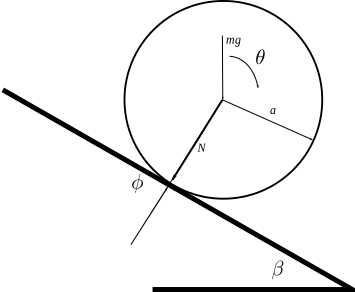
\includegraphics[width=0.45\textwidth]{rolling}
\caption{Layout}
\label{fig:rolling}
\end{subfigure}
\\
\begin{subfigure}[b]{0.95\textwidth}
\centering
\includegraphics[width=\textwidth]{DEM_Validation}
\caption{Accumulated disk rotation at t = 0.2~\si{\s} versus friction angle 
($\beta$=45\si{\degree}).}
\label{fig:DEM_Validation}
\end{subfigure}
\caption{Validation of DEM using a disk rollind down an inclined plane}
\label{fig:Validation_DEM}
\end{figure}

\begin{table}[tbhp]
\caption{Comparison of theoretical and DEM result for a disk on an inclined 
plane of 45\si{\degree}}
\label{table:dem_validation}
\centering
\begin{tabular}{lcccc}
\toprule
\multicolumn{5}{c}{$\phi$ = 0\si{\degree} (sliding)} \\ \midrule
 & $N=N/(Mg\cos\beta)$ & $S=S/(Mg)$ & $\ddot{a}/g$ & $\ddot{\theta}/g$\\
Theoretical~\citep{Ke1995} & 1.000 & 0.000 & 0.7071 & 0.000 \\
DEM & 1.000 & 0.000 & 0.7071 & 0.000 \\
\bottomrule
\end{tabular}
\end{table}

%%*******************************************************************************
\subsection[Cumulative beta distribution]{Cumulative $\beta$ distribution}

During a granular-metric analysis, the sample mush be representative of the 
grain properties including the particle size distribution (PSD) both in volume 
(mainly for the smallest particles) and in number (for the largest particles). 
This representativeness of PSD is a condition for a sample to be a 
representative volume element. However, this condition cannot be satisfied in 
DEM for a polydisperse sample, due to the upper limit on the computation 
capacity. It is important to extract a discrete ensemble of grain sizes such 
that a statistical representation of the size classes is 
obtained~\citep{Radjai2011}.

The $\beta$ distribution in its cumulative form is able to satisfactorily model 
the size span (ratio of the largest to the smallest grain) and the shape 
descriptor (relative weights of the maximum and the minimum grain sizes). The 
cumulative $\beta$ distribution ~\citep{Voivret2007} is defined as
%
\begin{equation}
\beta(x,a,b) = \frac{1}{\beta (a,b)}\int\limits_{0}^{x}t^{a-1}(1-t)^{b-1}dt \,,
\end{equation}
%
where a > 0 and b > 0 are the two parameters of the distribution. The 
\textit{B(a,b)} function is given by
%
\begin{equation}
B(a,b) = \frac{\Gamma(a)\Gamma(b)}{\Gamma(a+b)} \,,
\end{equation}
%
where $\Gamma$ is the gamma function defined by
%
\begin{equation}
\Gamma(x) = \int\limits_{0}^{\infty}t^{x-1}e^{-t}dt \,.
\end{equation}

The cumulative $\beta$ (CB) distribution is defined and normalised in the 
interval [0,1] with $\beta(0) = 0$ and  $\beta(1) = 1$. To represent the 
grading curve of grain size range $[d_{min},d_{max}]$ with CB, the argument 
\textit{x} is replaced by the reduced diameter $d_r$
%
\begin{equation}
d_r(d) = \frac{d - d_{min}}{d_{max} - d_{min}} \,,
\end{equation}
%
which varies in the range of [0,1]. The model grading curve $h(d)$ is given by 
the CD distribution in terms of the reduced diameters as
%
\begin{equation}
h(d,a,b) = \beta(d_r(d);a,b) \,.
\end{equation}

The parameters \textit{a} and \textit{b} of the CB model allows the shape 
descriptor $h(d)$ to vary easily. The size span is characterised by the ratio $ 
r = d_{max}/d_{min}$. The size span can also be defined as
%
\begin{equation}
s = \frac{d_{max}-d_{min}}{d_{max}+d_{min}} \,.
\end{equation}

A value of \textit{s} = 0 indicates a strictly mono-disperse grain size and a 
value of \textit{s} = 1 indicates an infinitely poly-disperse grain size 
distribution.~\citet{Voivret2007} observed a well graded particle size 
distribution for \textit{a} > 1 and \textit{b} > 1. 

In the present study, a value of \textit{a} = 4 and \textit{b} = 4 is adopted 
to get a well graded curve. In the present study, samples with different 
poly-dispersity \textit{r} = 1.5, 1.8, 2 and 6 are used.~\Cref{fig:DEM_Sample} 
shows a poly-disperse sample $r = 1.5$ generated using the CB method, for 
\textit{a} = 4 and \textit{b} = 4. The PSD curve of the generated 
sample is also presented.

%%*******************************************************************************

\subsection{Particle assembling methods}
In order to simulate a granular assembly, it is essential to assign an initial 
position and velocity to all the grains in the system. Particle positions 
should be chosen to be compatible to the structure (granular fabric) we are 
trying to simulate. In any event, the grains should not be positioned such that 
there is an appreciable overlap between grains. In order to achieve the initial 
position of the grains, various grain-assembling methods can be adopted. The 
grain assembling methods can be classified into two broad categories: 
dynamic methods and geometrical approaches. The dynamic approach involves 
packing of grains using laws of mechanics and contacts, while in the 
geometrical method the grains are packed considering their geometry, 
i.e. grain size, shape and its position. In general, the packing of grains can 
be categorized into two types: crystal/lattice packing, like hexagonal or 
square pattern of mono-disperse grains, and random packing with varying density 
employing mono-disperse or poly-disperse grains. The crystalline packing 
arrangements, such as hexagon and square lattices, are easier to generate, 
however they have non-trivial effects on the response of the granular 
system~\citep{Staron2005}. Hexagonal packing is the densest possible 
arrangement for mono-dispersed spherical grains. In 2D, the packing of 
mono-dispersed circles on a hexagonal lattice yields a packing density of 
$\eta_{\mathit{h}}=\frac{1}{6}\pi\sqrt{3}\approx 0.9068$



The rheology of a granular material is controlled by the geometry of the 
assembly, which includes the grain shape, size distribution, and their 
arrangement. This prevailing role of geometry sometimes permits to simplify the 
dynamics in favour of a better description of the geometry 
and/or higher numerical efficiency~\citep{Radjai2011}. For example, dense 
granular packing may be efficiently constructed by replacing the equations of 
dynamics by simple displacement rules satisfying the geometrical constraints. 
Purely geometrical procedures can be much simpler and numerically faster than 
dynamic or quasi-static methods. Contrary to dynamic simulation methods, 
the geometrical methods allow for quick assembling of a large number of 
grains. Such packing may then be used as the initial state for dynamic 
simulations. The issue of the assembling methods is to construct configurations 
of grains as close as possible to a state of mechanical equilibrium with 
built-in packing properties. This can be a target packing density for a 
given grain size distribution. In the same way, the average connectivity of the 
grains (coordination number) and the anisotropy of the contact network are 
basic geometrical properties. The coordination number represents the mechanical 
response of packing. The homogeneity of the grain assembly in terms of 
packing fraction and connectivity is another important property, which depends 
on the assembling rules. In the present study, the initial grain packing is 
obtained using the ballistic deposition technique.

\subsubsection{Ballistic deposition}
Initially a random arrangement of grains which do not touch each other is 
generated. The radii of the grains are chosen from the 
interval of $(\mathit{R}_{\mathit{min}},\mathit{R}_{\mathit{max}})$ in such a 
way that the total mass of all grains from a certain size interval is the same 
for all sizes, thus ensuring that neither larger nor smaller grains dominate 
the system. 
%This distribution can be obtained, if the radii are 
%chosen according to the probability distribution
%%
%\begin{equation}
%\mathit{p}(\mathit{R})=\frac{\mathit{R}_{\mathit{min}}\mathit{R}_{\mathit{max}}}{\mathit{R}_{\mathit{max}}
% - \mathit{R}_{\mathit{min}}} \frac{1}{\mathit{R}^{2}} \,.
%\end{equation}
%%
%Random numbers according to the above distribution can be generated from 
%equi-distributed random numbers $\mathit{z}\in [0,1]$ via the transformation
%%
%\begin{equation}
%\mathit{R}=\frac{\mathit{R}_{\mathit{min}}\mathit{R}_{\mathit{max}}}{\mathit{R}_{\mathit{max}}
% - z(\mathit{R}_{\mathit{max}} - \mathit{R}_{\mathit{min}})}  \,.
%\end{equation}
%%
The 
grains are arranged randomly on a regular lattice. In the second step, the 
grains arranged in a regular lattice are allowed to fall down maintaining a 
constant potential head between layers of grains (\cref{fig:ini_sample}). 
%
%and are 
%packed using the \textit{random deposition with relaxation method}, a 
%ballistic 
%deposition technique (\cref{fig:ini_sample}). 
%
%The geometrical methods help in 
%this way to improve 
%numerical efficiency in the preparation phase. For example, gravitational 
%deposition of grains located initially on a regular grid can require hours of 
%computation whereas a nearly similar result may be obtained by means of a 
%geometrical method in only a few minutes. The drawback is that the resulting 
%sample will not be in mechanical equilibrium and no information is available 
%on 
%the contact forces. Nevertheless, depending on the relaxation rule, the sample 
%may still be sufficiently close to equilibrium to be considered as a good 
%starting point for mechanical simulations. Hence, a combined approach of 
%ballistic deposition and Discrete Element Method is adopted in the present 
%study to generate mechanically stable samples. 

\begin{figure}
	\centering
	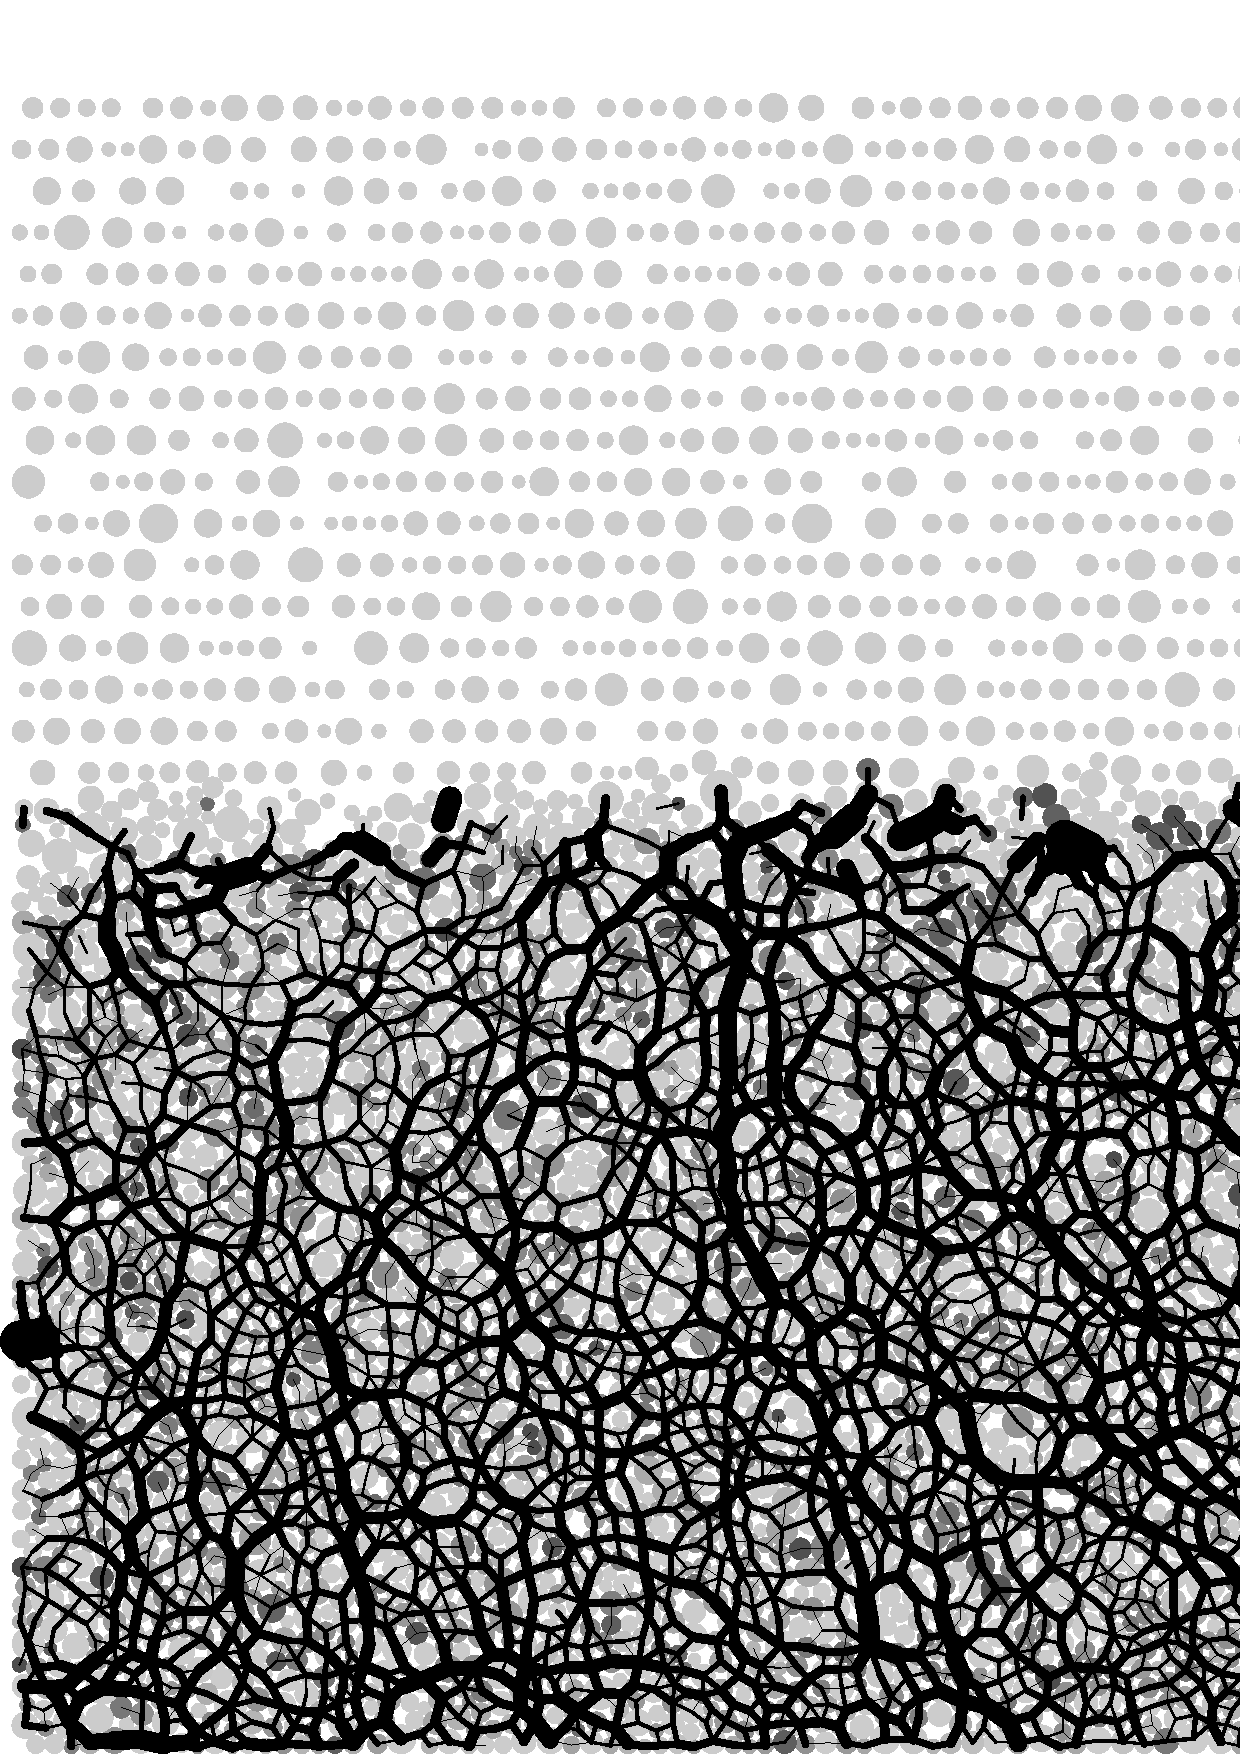
\includegraphics[width=0.75\textwidth]{ini_sample}
	\caption{Generation of a poly-disperse sample using ballistic deposition 
	technique}
	\label{fig:ini_sample}
\end{figure}
%
%The random deposition and 
%relaxation method, first proposed by~\citet{vold1959a} and developed 
%by~\citet{jullien1992} and \citet{meakin1985}, is adopted in the present 
%study. 
%The general principle of this method is quite simple 
%(\cref{fig:ballistic}); it consists of placing the grains consecutively on 
%a substrate or a layer of already deposited grains. Each grain first 
%touches the substrate or a deposited grain, then undergoes a relaxation 
%process 
%(single-grain restructuring) along the steepest descent (steepest-descent 
%model) until a more stable position according to a stability criterion is 
%reached. 

The construction of the packing proceeds layer by layer from the 
substrate, hence this deposition model is also known as bottom-to-top 
restructuring model. 
%
%The first step is to release a grain from a random 
%position above the substrate. Upon contact with the first deposited grain, the 
%grain rolls following the steepest descent until a new contact is formed with 
%a second grain.
%
In 2D, two contacts are sufficient to balance a grain if its 
centre of gravity lies between the two contacts. This corresponds to a position 
of local stable equilibrium. 
%If this criterion is not met, the grain continues 
%to roll and the procedure is iterated until a local stable position is 
%reached. 
%~\Cref{fig:ballistic} shows a schematic view of the ballistic deposition 
%technique  (the grey grains are periodic images of the black ones).
In this method, the order of deposited grains is generally random and 
independent of their sizes. The mechanically stable sample obtained from this 
method is presented in~\cref{fig:DEM_Sample_r6}. 
Dense granular samples are prepared with zero initial friction angle. Zero 
frictional resistance ensures the densest possible packing. The friction angle 
is turned on during the analysis. To generate a dense sample, the sample is 
subjected to vibrations at varying frequencies. 

\begin{figure}[htbp]
\centering
%	\begin{subfigure}[b]{0.95\textwidth}
%	\centering
%	\includegraphics[width=0.975\textwidth]{ballistic}
%	\caption{\textit{Ballistic deposition}: first contact followed by 
%	steepest descent and small-scale periodic sample~\citep{Radjai2011}}
%	\label{fig:ballistic}
%	\end{subfigure} \\
%	\begin{subfigure}[b]{0.95\textwidth}
%	\centering
	\includegraphics[width=0.975\textwidth]{DEM_Sample_r6}
	\caption{A poly-dispersed DEM sample generated using ballistic deposition 
	technique}
	\label{fig:DEM_Sample_r6}
%	\end{subfigure} \\
%\caption{Ballistic deposition}
%\label{fig:ballistic_sample}
\end{figure}

Although, there is no optimum specimen generation 
technique~\citep{OSullivan2011}, there is a need to assess the homogeneity of 
the packing density generated~\citep{Jiang2003}. The homogeneity of the sample 
is assessed by measuring the void-ratio within sub-volumes. The generated 
specimen is discretised into horizontal bands of $2.5d_{50}$. The homogeneity 
of the packing is calculated by the variance \textit{S} in the void ratio.
%
\begin{equation}
S=\frac{1}{N_{layer}-1}\sum\limits_{i=1}^{N_{layer}}(e - e_i)^2 \,,
\end{equation}
%
where $N_{layer}$ is the number of layers and \textit{e} is the overall void 
ratio. A variance \textit{S} of 2.74\% is observed, which is less than 
5\%~\citet{Jiang2003}, indicating a homogeneous sample.


\subsection{Voronoi tessellation}

In order to extract bulk properties, such as packing density, stresses and 
strains, from a DEM simulation, it is important to quantify the granular 
texture. A useful geometrical representation of granular texture consists of 
dividing the space occupied by the particles into contiguous cells. This 
procedure is called `tessellation'. Voronoi tessellation is one of the mostly 
commonly used technique. For a finite set of points $p_1, \dots, p_n$ in the 
Euclidean space, the domain/plane is discretised into convex polygons such that 
each polygon contains exactly one point $p_i$ and every point in a given 
polygon is closer to its generating point $p_i$ than to any other. The inverse 
of the Voronoi tessellation is the Delaunay triangulation.

In the present study, the~\citet{Fortune1992} sweep line algorithm is 
implemented to 
tessellate the region surrounding each grain in the geometry. Once each grain 
has a corresponding area, the macroscopic properties such as the bulk density 
and stresses can be extracted from micro-mechanical properties such as the 
local packing density and force chains.

Fortune sweep line algorithm involves a sweep line and a beach line, both of 
which move through the plane from left to right as the algorithm progresses. 
The sweep line is a straight line which moves from left to right across the 
plane. At any time during the algorithm, the points (grains) to the left of the 
sweep line will be incorporated into a Voronoi cell. While the points on the 
right of the sweep line are yet to be considered. The beach line is a complex 
curve, composed of pieces of parabolas that divides the plane within which the 
Voronoi diagram is known. As the sweep line crosses a point, a parabola 
evolves from the generating point. As the sweep line progresses, the 
vertices of the beach line, at which two parabolas cross, trace out the edges 
of the Voronoi diagram. The beach line progresses by keeping each parabola base 
exactly half way between the points initially swept over with the sweep line, 
and the new position of the sweep line.~\Cref{fig:sweep_voro} shows the Fortune 
sweep line algorithm in progress. In the present study, a modified version of 
the sweepline algorithm is used to construct an additively weighted Voronoi 
diagram, in which the distance to each site (grain) is offset by the weight of 
the site, i.e., the radius of the grain.

\begin{figure}[tbhp]
\centering
\includegraphics[width=0.9\textwidth]{sweep_voro}
\caption[Fortune sweep line algorithm for generating Voronoi 
Tesselation]{Fortune sweep line algorithm for generating Voronoi Tesselation. 
Generated from \url{http://www.diku.dk/hjemmesider/studerende/duff/Fortune/}.}
\label{fig:sweep_voro}
\end{figure}

The Voronoi tessellation is used to study the evolution of packing fraction 
during the collapse of a granular column.~\Cref{fig:tessellation} shows the 
Voronoi tessellation of the run-out for a granular column with an initial 
aspect ratio of 6 at time $t = 3 \tau_c$. The distribution of local packing 
density for the run-out is shown in~\cref{fig:local_density}. Dark regions 
represent dense packing, while loose regions are shown in white. The run-out at 
this stage has a bulk packing density of 81.23\%. It is difficult to tessellate 
the free surface and the Voronoi cells on the free surface do not represent the 
actual packing density. Hence, during the evaluation of the macroscopic 
density, the packing density of surface grains that are larger than a threshold 
value are ignored. Voronoi Tessellation is a useful tool to extract continuum 
properties from DEM simulations. In the present study, the Voronoi tessellation 
is used to understand the evolution of packing density and entrainment of water 
in the flow front (due to hydroplaning) in granular flows.

\begin{figure}[tbhp]
\centering
\begin{subfigure}[b]{0.95\textwidth}
\centering
\includegraphics[width=\textwidth]{tessellation}
\caption{Voronoi Tessellation}
\label{fig:tessellation}
\end{subfigure}
\\
\begin{subfigure}[b]{0.95\textwidth}
\centering
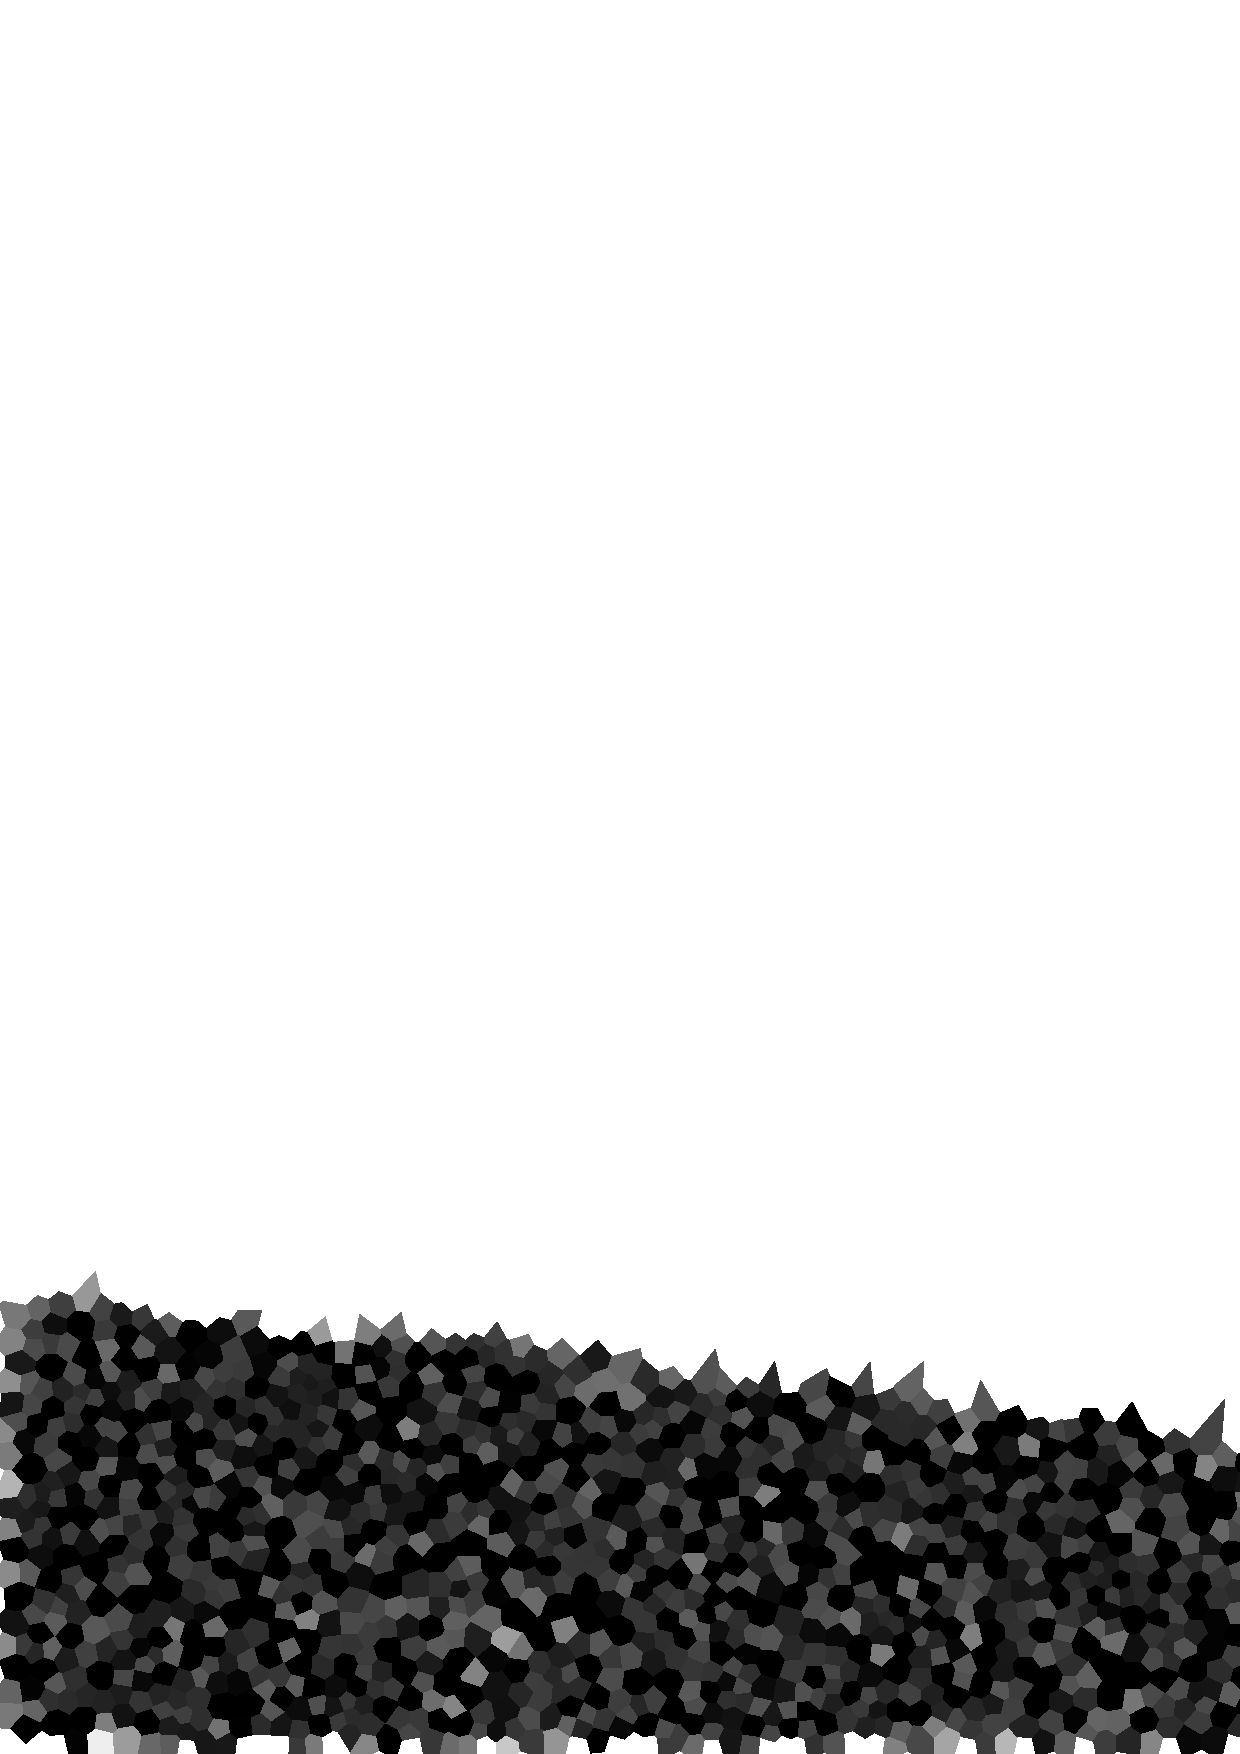
\includegraphics[width=\textwidth]{local_density}
\caption{Local packing density (dark - dense and light - loose)}
\label{fig:local_density}
\end{subfigure}
\caption{Voronoi tessellation of a run-out profile showing the local packing 
density}
\label{fig:voronoi_tesselation}
\end{figure}

\section{Summary}

A plane-strain Material Point Method is implemented in the present study to 
describe the continuum response of granular flows. The Generalised 
Interpolation Material Point GIMP method is implemented to minimize 
oscillations in large-deformation problems due to cell-crossing noise. The 
effect of mesh size and the number of material points per cell on the run-out 
behaviour is also investigated. The accuracy of the continuum approach improves 
with increase in the number of material points per cell and a decrease in the 
mesh size. The grain-scale response is captured using a 
two-dimensional DEM code. The discrete grains are generated using a cumulative 
$\beta$ distribution, which mimics the particle size distribution curves. The 
sample is generated using the ballistic deposition technique and the 
homogeneity of the generated sample is verified by investigating the variance 
in the void-ratio at different layers. A sweep-line Voronoi tessellation 
approach is adopted to extract macroscopic parameters such as stresses and 
packing density from micro-scale properties such as the local packing fraction. 
These multi-scale tools are used to understand the rheophysics of
dry granular flows and to evaluate the suitability of MPM as a continuum 
approach in modelling granular flow behaviour.